\documentclass[a4paper,twoside]{article}
\usepackage[T1]{fontenc}
\usepackage[bahasa]{babel}
\usepackage{graphicx}
\usepackage{graphics}
\usepackage{float}
\usepackage[cm]{fullpage}
\pagestyle{myheadings}
\usepackage{etoolbox}
\usepackage{setspace} 
\usepackage{lipsum} 
\usepackage{amsmath}
\setlength{\headsep}{30pt}
\graphicspath{{./Gambar/}}% folder tempat gambar 
\usepackage{amsthm}
\newtheorem{theorem}{Teorema}
\usepackage{algorithm,amsmath,algpseudocode}%pseudocode in latex
\usepackage[skins]{tcolorbox}
\usepackage{listings}
\usepackage[inner=2cm,outer=2.5cm,top=2.5cm,bottom=2cm]{geometry} %margin
\usepackage{changepage}
% \pagestyle{empty}

\makeatletter
\renewcommand{\@maketitle} {\begin{center} {\LARGE \textbf{ \textsc{\@title}} \par} \bigskip {\large \textbf{\textsc{\@author}} }\end{center} }
\renewcommand{\thispagestyle}[1]{}
\markright{\textbf{\textsc{Laporan Perkembangan Pengerjaan Skripsi\textemdash Sem. Genap 2019/2020}}}

\onehalfspacing
 
\begin{document}

\title{\@judultopik}
\author{\nama \textendash \@npm} 

%ISILAH DATA BERIKUT INI:
\newcommand{\nama}{Stephen Jordan}
\newcommand{\@npm}{2016730018}
\newcommand{\tanggal}{02/05/2020} %Tanggal pembuatan dokumen
\newcommand{\@judultopik}{Penerapan Algoritma Anonimisasi Pada Lingkungan Big Data} % Judul/topik anda
\newcommand{\kodetopik}{MTA4801}
\newcommand{\jumpemb}{2} % Jumlah pembimbing, 1 atau 2
\newcommand{\pembA}{Mariskha Tri Adithia, P.D.Eng}
\newcommand{\pembB}{Dr. Veronica Sri Moertini, Ir., M.T.}
\newcommand{\semesterPertama}{48 - Genap 19/20} % semester pertama kali topik diambil, angka 1 dimulai dari sem Ganjil 96/97
\newcommand{\lamaSkripsi}{1} % Jumlah semester untuk mengerjakan skripsi s.d. dokumen ini dibuat
\newcommand{\kulPertama}{Skripsi 1} % Kuliah dimana topik ini diambil pertama kali
\newcommand{\tipePR}{B} % tipe progress report :
% A : dokumen pendukung untuk pengambilan ke-2 di Skripsi 1
% B : dokumen untuk reviewer pada presentasi dan review Skripsi 1
% C : dokumen pendukung untuk pengambilan ke-2 di Skripsi 2

% Dokumen hasil template ini harus dicetak bolak-balik !!!!

\maketitle

\pagenumbering{arabic}

\section{Data Skripsi} %TIDAK PERLU MENGUBAH BAGIAN INI !!!
Pembimbing utama/tunggal: {\bf \pembA}\\
Pembimbing pendamping: {\bf \pembB}\\
Kode Topik : {\bf \kodetopik}\\
Topik ini sudah dikerjakan selama : {\bf \lamaSkripsi} semester\\
Pengambilan pertama kali topik ini pada : Semester {\bf \semesterPertama} \\
Pengambilan pertama kali topik ini di kuliah : {\bf \kulPertama} \\
Tipe Laporan : {\bf \tipePR} -
\ifdefstring{\tipePR}{A}{
			Dokumen pendukung untuk {\BF pengambilan ke-2 di Skripsi 1} }
		{
		\ifdefstring{\tipePR}{B} {
				Dokumen untuk reviewer pada presentasi dan {\bf review Skripsi 1}}
			{	Dokumen pendukung untuk {\bf pengambilan ke-2 di Skripsi 2}}
		}
		
\section{Latar Belakang}
Berkembangnya penggunaan sistem informasi di jaman sekarang mengakibatkan data dihasilkan dalam jumlah yang sangat banyak. Data yang jumlahnya sangat banyak ini dikumpulkan dan disimpan dalam tabel basis data untuk keperluan analisis data di masa yang akan datang. Data yang dikumpulkan secara terus-menerus apabila tidak dilakukan analisis secara berkala, maka suatu saat nanti jika proses analisis data dilakukan, proses analisis tersebut berlangsung sangat lama karena ukuran datanya sudah terlanjur besar. Data yang terus bertumbuh menyebabkan basis data konvensional menjadi kurang efektif untuk mengolah data. Teknologi \textit{big data} digunakan untuk mengurangi biaya penyimpanan dan komputasi data, sehingga kapasitas data dapat ditingkatkan dan data berukuran besar menjadi lebih mudah untuk diolah.

{\it Big data} adalah kumpulan data dalam jumlah data yang sangat besar disimpan, diolah, dan dianalisis untuk menghasilkan informasi yang bermanfaat sebagai dasar pengambilan keputusan atau kebijakan. Karena \textit{big data} memiliki ukuran data yang besar, sehingga untuk melakukan analisis pada \textit{big data}, data yang sudah terkumpul akan dibagi ke beberapa komputer untuk diolah secara paralel. Konsep ini disebut sistem terdistribusi. Sistem terdistribusi adalah solusi dari pengolahan \textit{big data} karena terbukti dapat mengurangi biaya penyimpanan dan komputasi data karena dilakukan secara paralel. Untuk melakukan analisis data, diperlukan teknik khusus untuk mencari tahu pola apa saja yang terbentuk dari sekumpulan data yang telah dikumpulkan. Oleh karena itu, diperlukan teknik \textit{data mining} untuk melakukan analisis data.


{\it Data mining} adalah teknik yang diciptakan untuk melihat pola yang terbentuk dari sekumpulan data yang telah terkumpul dalam jumlah yang besar. {\it Data mining} terbukti efektif untuk menggantikan pemrosesan kueri pada basis data konvesional dalam kasus analisis \textit{big data}, karena basis data konvesional tidak menerapkan konsep sistem terdistribusi sehingga waktu komputasinya sangat lambat. Pemodelan data mining nantinya akan dijalankan pada sistem terdistribusi, sehingga waktu komputasi untuk analisis \textit{big data} dapat diminimalkan. Hasil \textit{data mining} nantinya akan dipakai untuk berbagai macam kebutuhan. Biasanya sebuah perusahaan akan meminta data dari perusahaan lain untuk kebutuhan analisis. Masalah yang umum terjadi adalah data hasil pengolahan \textit{data mining} banyak mengandung data yang bersifat privasi sehingga perlu adanya cara untuk menjamin perlindungan privasi pada data yang akan didistribusikan.

Perlindungan privasi untuk distribusi data dapat dicapai dengan menggunakan metode enkripsi dan anonimisasi pada hasil pengolahan data mining. Enkripsi adalah metode yang memanfaatkan pola atau kunci tertentu untuk melindungi data yang sifatnya sensitif. Anonimisasi adalah metode yang menyamarkan satu atau lebih nilai atribut data agar data seseorang tidak dapat saling dibedakan dengan data lainnya. Salah satu kekurangan dari metode enkripsi dibandingkan metode anonimisasi adalah keamanan enkripsi dapat diretas melalui penalaran hubungan nilai atribut yang unik untuk setiap baris data. Penalaran ini dicapai dengan menggabungkan seluruh nilai atribut yang unik pada masing-masing baris data untuk membentuk sebuah pola kelompok data. dPenalaran ini sangat berbahaya karena menghubungkan nilai atribut data yang secara tidak langsung dapat mengungkapkan entitas pemilik data. Dengan menerapkan konsep  anonimisasi diharapkan nilai keterhubungan antar atribut data diperkecil sehingga privasi dapat terlindungi

Dengan melakukan anonimisasi pada sebagian nilai atribut, bobot informasi yang diperoleh akan semakin kecil. Semakin kecil bobot informasi yang diperoleh maka pola untuk membentuk kelompok entitas data semakin kecil sehingga perlindungan privasi akan semakin aman. Akan tetapi dengan semakin kecil bobot informasi yang diperoleh maka nilai akurasi yang dihasilkan oleh metode anonimisasi akan semakin kecil. Oleh karena itu diperlukan cara untuk menyeimbangkan keamanan dan nilai akurasi informasi. Permasalahan {\it k-anonymity} adalah pencarian solusi untuk menyeimbangkan nilai akurasi informasi yang diperoleh dengan nilai informasi yang dilindungi. Permasalahan {\it k-anonymity} diuji dengan pendekatan generalisasi dan supresi. Hasilnya dinilai kurang efektif karena tingginya jumlah informasi yang hilang. Berdasarkan penelitian, permasalahan {\it k-anonymity} tercapai melalui penerapan {\it k-member clustering}. Penerapan {\it k-member clustering} pada algoritma {\it Greedy k-member clustering} dinilai baik karena dapat meminimalkan jumlah informasi yang hilang. Agar algoritma \textit{Greedy k-member clustering} dapat berjalan dengan waktu pemrosesan yang tidak terlalu lama, maka akan digunakan \textit{framework} Spark untuk mengatasi permasalahan \textit{big data}.

Spark adalah {\it framework} yang tepat untuk melakukan proses anonimisasi data pada lingkungan \textit{big data}, karena pekerjaan pengolahan data yang besar dapat dibagi ke beberapa komputer pada sistem terdistribusi. Penggunaan Spark dipilih karena Hadoop memiliki waktu pemrosesan \textit{big data} yang lebih lama dari Spark dengan melakukan komputasi pada \textit{hardisk}, sedangkan Spark melakukan komputasi pada memori. Selain itu Spark memiliki jenis \textit{library} yang lebih beragam dibandingkan dengan Hadoop. Spark  mampu melakukan pemrosesan teknik {\it data mining} pada lingkungan \textit{big data} menggunakan {\it library} tambahan yaitu Spark MLlib. Spark MLlib menfasilitasi pemodelan \textit{data mining} yaitu klasifikasi dan pengelompokan/\textit{clustering}. Kekurangan dari Spark adalah tidak mempunyai penyimpanan yang tetap, sehingga membutuhkan  mekanisme penyimpanan Hadoop, agar hasil pemrosesan data dapat tersimpan di dalam {\it hardisk} komputer.

Pada skripsi ini, akan dibuat dua jenis perangkat lunak yaitu perangkat lunak untuk anonimisasi data dan perangkat lunak untuk analisis data. Perangkat lunak anonimisasi data menggunakan konsep {\it k-anonimity} dengan implementasi algoritma \textit{Greedy k-member clustering} agar sebuah data tidak dapat dibedakan dengan $k-1$ data lainnya. Perangkat lunak anonimisasi data dibuat dengan bahasa Scala dan berjalan di atas Spark untuk meminimalkan waktu komputasi pada proses anonimisasi di lingkungan {\it big data}. Algoritma {\it Greedy k-member clustering} dinilai tepat untuk melakukan pengelompokan data karena meminimalkan jumlah informasi yang hilang saat proses {\it data mining} yang terbukti pada penelitian sebelumnya. Kedua jenis perangkat lunak ini menerima data input dalam format CSV. Untuk tampilannya, kedua jenis perangkat lunak akan dibuat menggunakan GUI dari \textit{library} Scala-swing. Penelitian ini memiliki tujuan utama yaitu membandingkan nilai akurasi dari hasil {\it data mining} sebelum dan setelah dilakukan anonimisasi.

\section{Rumusan Masalah}
Berdasarkan latar belakang di atas, rumusan masalah pada skripsi ini adalah sebagai berikut:
\begin{enumerate}
\item Bagaimana cara kerja algoritma {\it Greedy k-member clustering} ?
\item Bagaimana implementasi algoritma {\it Greedy k-member clustering} pada Spark?
\item Bagaimana hasil {\it data mining} sebelum dan setelah dilakukan anonimisasi?
\end{enumerate}

\newpage
\section{Tujuan}
Berdasarkan rumusan masalah di atas, tujuan pada skripsi ini adalah sebagai berikut:
\begin{enumerate}
\item Mempelajari cara kerja algoritma {\it Greedy k-member clustering}.
\item Mengimplementasikan algoritma {\it Greedy k-member clustering } pada Spark.
\item Menganalisis hasil {\it data mining} sebelum dan setelah dilakukan anonimisasi.
\end{enumerate}

\section{Detail Perkembangan Pengerjaan Skripsi}
Detail bagian pekerjaan skripsi sesuai dengan rencana kerja/laporan perkembangan terakhir:
	\begin{enumerate}
		\item \textbf{Melakukan studi literatur mengenai teknik-teknik dasar data mining}\\
		{\bf Status :} Ada sejak rencana kerja skripsi.\\
		{\bf Hasil :} Data yang dikumpulkan bertambah banyak, sehingga perlu adanya cara untuk melakukan proses ekstraksi informasi pada sekumpulan data yang sangat banyak. Menurut Gartner, \textit{data mining} adalah proses menemukan korelasi, pola, dan tren baru yang bermakna dengan menyaring sejumlah besar data yang disimpan menggunakan teknologi pengenalan pola serta teknik statistik dan matematika. \textit{Data mining} merupakan bagian dari \textit{Knowledge Discovery in Databases} (KDD). KDD adalah proses transformasi sekumpulan data yang disimpan pada basis data menjadi informasi yang berguna.\\

\begin{figure}[H]
	\centering
	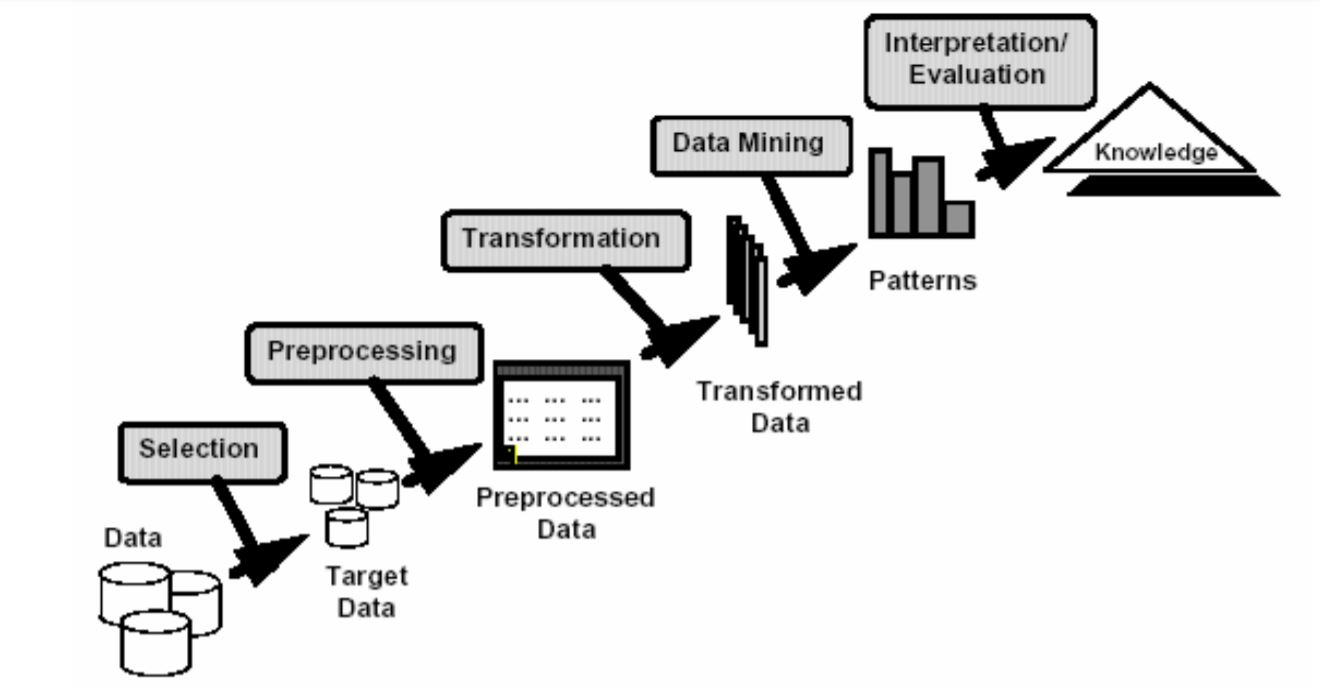
\includegraphics[scale=0.4]{datamining1}
	\caption{Tahapan pada KDD}
	\label{fig:datamining1}
\end{figure}

\noindent Berikut ini adalah penjelasan tahapan pada KDD pada Gambar \ref{fig:datamining1} sebagai berikut:

\begin{enumerate}
\item \textit{Selection}: proses mengambil data yang relevan terhadap analisis.
\item \textit{Preprocessing}: proses pembersihan data dari data yang tidak konsisten dan integrasi data saat penggabungan data.
\item \textit{Transformation}: proses manipulasi data menggunakan konsep agregasi, generalisasi, normalisasi, dan reduksi untuk kebutuhan analisis.
\item \textit{Data mining}: proses ekstraksi informasi menggunakan metode pengenalan pola seperti klasifikasi, pengelompokan/\textit{clustering}.
\item \textit{Interpretation/evaluation}: proses interpretasi hasil pengolahan data menjadi sebuah grafik yang dapat dimengerti.
\end{enumerate}

\textbf{Klasifikasi}
			
Klasifikasi adalah proses menemukan model (atau fungsi) yang cocok untuk mendeskripsikan dan membedakan sebuah kelas data dengan kelas data lain. Dalam pembelajaran mesin, klasifikasi sering dianggap sebagai contoh dari metode pembelajaran yang diawasi, yaitu menyimpulkan fungsi dari data pelatihan berlabel.\\


\textbf{Naive Bayes}
\par \textit{Naive Bayes} menerapkan klasifikasi dengan menggunakan metode probabilitas dan statistik. Pemodelan ini mencari nilai probabilitas tertinggi pada masing-masing kelas menggunakan teorema \textit{Bayes}. Kelas dengan probabilitas tertinggi akan dipilih sebagai hasil akhir. \textit{Naive Bayes} mudah untuk dibangun dan memiliki komputasi yang lebih cepat daripada model klasifikasi lainnya.\\

\noindent Teorema \textit{Bayes} menemukan probabilitas suatu peristiwa terjadi mengingat probabilitas peristiwa lain yang telah terjadi. Teorema \textit{Bayes} dinyatakan secara matematis melalui persamaan berikut:

\begin{equation}
P(H|D) = \frac{P(D|H) \cdot P(H)}{P(D)}
\end{equation}

\noindent
Dari perhitungan probabilitas teorema Bayes, akan dicari kelas dengan probabilitas maksimum. Probabilitas maksimum dapat dinyatakan secara matematis melalui persamaan berikut:

\begin{align}
MAP(H) = max(P(H|D))
\end{align}

\noindent Keterangan:
\begin{itemize}
\item $P(H|D)$ adalah probabilitas posterior apabila diberika hipotesis H dan diketahui data D. 
\item $P(D|H$) adalah probabilitas posterior data D jika hipotesis h adalah benar.
\item $P(H)$ adalah probabilitas hipotesis h adalah benar 
\item $P(D)$ adalah probabilitas data.
\end{itemize}

\vspace{0.3cm}

\noindent Gambar \ref{fig:naive_bayes1} diberikan untuk menggambarkan kondisi cuaca saat bermain golf. Masing-masing data dikategorikan berdasarkan nilai atribut \textit{PlayGolf}, yaitu cocok (\textit{Yes}) atau tidak cocok (\textit{No}). 

\begin{figure}[H]
	\centering
	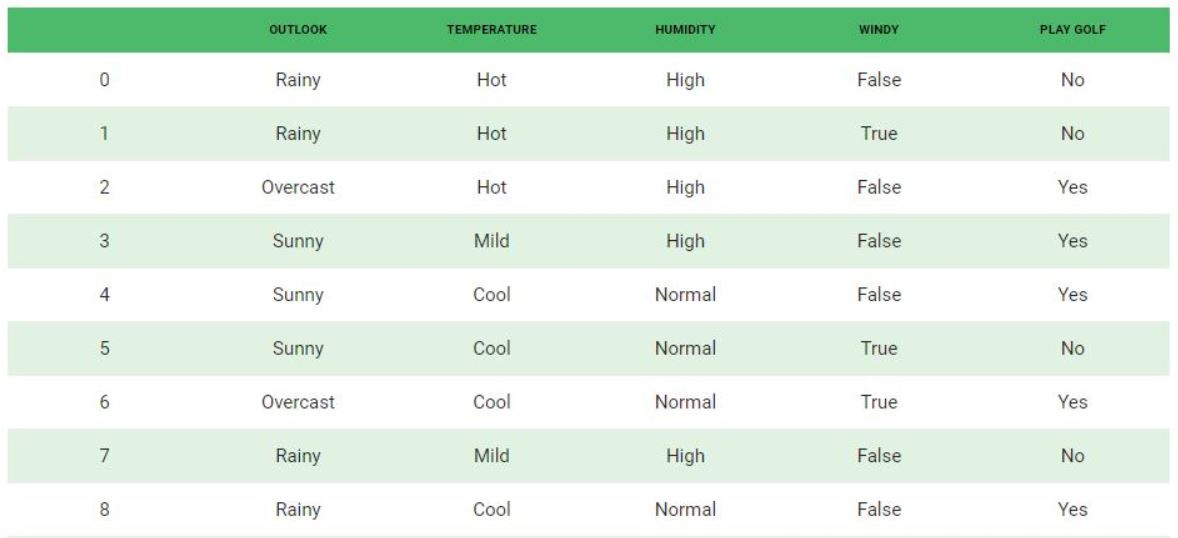
\includegraphics[scale=0.6]{naive_bayes1}
	\caption{Dataset Kondisi Cuaca Bermain Golf}
	\label{fig:naive_bayes1}
\end{figure}

\noindent Berikut adalah pengelompokan nilai berdasarkan dataset yang telah diberikan:

\begin{itemize}

\item 
Vektor fitur\\
Vektor fitur adalah vektor yang mewakili nilai fitur untuk setiap baris dataset. Vektor fitur dalam dataset ini tersusun dari nilai atribut \textit{Outlook, Temperature, Humidity, dan Windy}.

\item
Vektor respon\\
Vektor respon adalah nilai prediksi kelas untuk setiap vektor fitur. Vektor Respon dalam dataset ini diwakili oleh nilai atribut \textit{PlayGolf}.

\end{itemize}


\noindent Secara singkat, langkah kerja algoritma \textit{Naive Bayes} dapat dijelaskan sebagai berikut:

\begin{enumerate}
\item Merepresentasikan teorema Bayes terhadap vektor fitur.\\
Berdasarkan dataset, teorema Bayes dapat diubah seperti berikut:

\begin{equation}
P(y|X) = \frac{P(X|y) \cdot P(y)}{P(X)}
\end{equation}

Di mana y adalah variabel kelas dan X adalah vektor fitur (dengan ukuran n), dinyatakan melalui persamaan berikut:

\begin{equation}
X = (x_1, x_2, x_3, \ldots, x_n)
\end{equation}

Contoh: $X = (Rainy, Hot, High, False)$, $y = No$
\\\\
Diasumsikan teorema \textit{Bayes} saling independen terhadap fitur-fiturnya. Berikut adalah persamaan teorema \textit{Bayes} baru, jika memakai lebih dari satu nilai atribut:

\begin{equation}
P(y|x_1,\ldots,x_n) = \frac{P(x_1|y) P(x_2|y) \ldots P(x_n|y) P(y)}{P(x_1) P(x_2) \ldots P(x_n)}
\end{equation}


\item Gambar \ref{fig:naive_bayes2} adalah contoh menghitung probabilitas masing-masing atribut.

\begin{figure}[H]
	\centering
	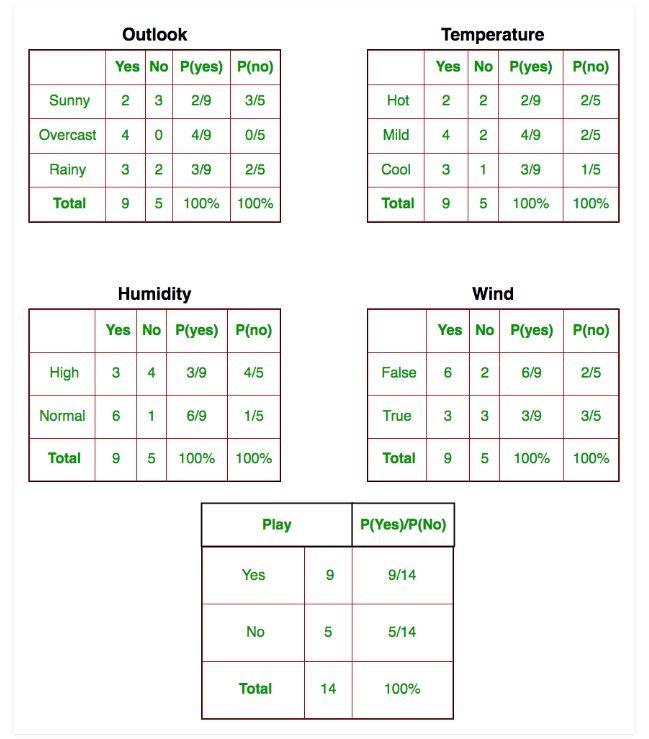
\includegraphics[scale=0.55]{naive_bayes2}
	\caption{Menghitung Probabilitas}
	\label{fig:naive_bayes2}
\end{figure}

Contoh: menghitung $P(No)$ untuk nilai \textit{Sunny} pada atribut \textit{Outlook}
\begin{equation}
P(No) = \frac{frekuensi(Sunny \cap No)}{frekuensi(No)}
\end{equation}

Contoh: menghitung $P(Yes)$ untuk nilai \textit{Sunny} pada atribut \textit{Outlook}
\begin{equation}
P(Yes) = \frac{frekuensi(Sunny \cap Yes)}{frekuensi(Yes)}
\end{equation}

\item Menghitung probabilitas bersyarat jika diketahui nilai dari data baru. \\\\
Contoh: \textit{today = (Sunny, Hot, Normal, False)}
\begin{figure}[H]
	\centering
	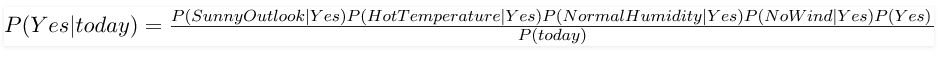
\includegraphics[scale=0.73]{naive_bayes3}
	\label{fig:naive_bayes3}
\end{figure}

\begin{equation}
P(Yes|today) = \frac{3}{5} \cdot \frac{2}{5} \cdot \frac{1}{5} \cdot \frac{2}{5} \cdot \frac{5}{14} = 0.0068
\end{equation}

\begin{figure}[H]
	\centering
	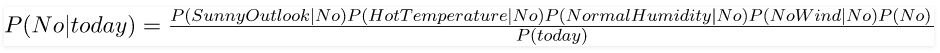
\includegraphics[scale=0.73]{naive_bayes4}
	\label{fig:naive_bayes4}
\end{figure}

\begin{equation}
P(No|today) = \frac{2}{9} \cdot \frac{2}{9} \cdot \frac{6}{9} \cdot \frac{6}{9} \cdot \frac{9}{14} = 0.0068
\end{equation}

\item Melakukan normalisasi terhadap probabilitas besyarat.\\

Setelah probabilitas bersyarat dinormalisasi, akan menjadi seperti berikut:

\begin{equation}
P(Yes|today) = \frac{0.0141}{0.0141 + 0.0068} = 0.67
\end{equation}

\begin{equation}
P(No|today) = \frac{0.0068}{0.0141 + 0.0068} = 0.33
\end{equation}

Sehingga memiliki probabilitas total seperti berikut:

\begin{equation}
P(Yes|today) + P(No|today) = 1
\end{equation}

\item Mencari probabilitas tertinggi.\\

Berdasarkan pernyataan berikut:
\begin{equation}
P(Yes|today) > P(No|today)
\end{equation}

\noindent Dapat disimpulkan bahwa, jika diberikan data dengan nilai \textit{(Sunny, Hot, Normal, False)} klasifikasi yang tepat untuk atribut \textit{PlayGolf} adalah \textit{Yes}.

\end{enumerate}

\newpage
\textbf{Pengelompokan/Clustering} 

\textit{Clustering} adalah salah satu teknik analisis data yang paling umum digunakan untuk mendapatkan kemiripan antar data. \textit{Clustering} dapat didefinisikan sebagai sebuah tugas untuk mengidentifikasi subkelompok dalam data sedemikian rupa sehingga titik data dalam subkelompok/\textit{cluster} yang sama sangat mirip sedangkan titik data dalam kelompok berbeda sangat berbeda. Contoh pemodelan \textit{clustering} adalah \textit{K-Means}.

\textbf{K-Means} 

\textit Algoritma \textit{k-means} adalah algoritma pembelajaran mesin \textit{unsupervised learning} untuk menentukan objek tersebut benar-benar milik kelompok data tertentu. \textit{Unsupervised learning} artinya tidak ada label yang ditentukan dalam data. Gagasan utama \textit{k-means} adalah menetapkan setiap data ke dalam cluster dengan mean terdekat (centroid). Mencari titik terdekat dilakukan dengan cara menghitung distance antara dua data menggunakan Euclidean distance, lalu membandingkat titik yang memiliki jarang paling dekat dengan titik lainnya. \\

\noindent Berikut adalah persamaan untuk menghitung \textit{Euclidean distance}:
\begin{equation}
EuclidDist(p_i,C_i) = \sqrt[]{(p_1-C_1)^2+(p_2-C_2)^2+\ldots +(p_n-C_n)^2}
\end{equation}

\noindent Gambar \ref{fig:kmeans_1} adalah skor A dan B untuk masing-masing individu:

\begin{figure}[H]
	\centering
	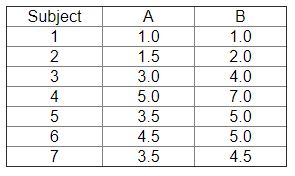
\includegraphics[scale=0.9]{kmeans_1}
	\caption{Contoh Dataset K-Means}
	\label{fig:kmeans_1}
\end{figure}

\noindent Secara singkat, langkah kerja algoritma \textit{k-means} dapat dijelaskan sebagai berikut:
\begin{enumerate}

\item Gambar \ref{fig:kmeans_2} adalah hasil pengelompokan awal untuk $k = 2$. Untuk menentukan titik \textit{centroid} awal, akan dicari nilai A dan B terjauh dengan data lainnya menggunakan \textit{Euclidean distance}.

\begin{figure}[H]
	\centering
	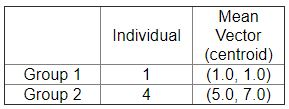
\includegraphics[scale=0.9]{kmeans_2}
	\caption{Hasil Pengelompokan Awal}
	\label{fig:kmeans_2}
\end{figure}

\item Data yang tersisa akan diperiksa secara berurutan dan dialokasikan pada \textit{cluster} yang paling dekat dengan \textit{centroid} awal menggunakan \textit{Euclidean distance}. Gambar \ref{fig:kmeans_3} menunjukan vektor rata-rata (\textit{centroid}) akan dihitung ulang setiap kali anggota baru ditambahkan.

\begin{figure}[H]
	\centering
	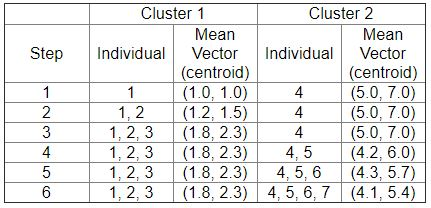
\includegraphics[scale=0.9]{kmeans_3}
	\caption{Mencari Centroid Kelompok}
	\label{fig:kmeans_3}
\end{figure}

\item Menentukan titik \textit{centroid} baru pada \textit{cluster} yang baru terbentuk dari tahap sebelumnya.

\begin{figure}[H]
	\centering
	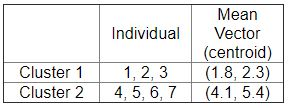
\includegraphics[scale=0.9]{kmeans_4}
	\caption{Hasil Pengelompokan Baru}
	\label{fig:kmeans_4}
\end{figure}

\item Belum bisa dipastikan bahwa setiap individu telah dialokasikan pada cluster yang tepat. Oleh karena itu, perlu membandingkan \textit{distance} masing-masing data dengan \textit{centroid} baru pada masing-masing kelompok. Gambar \ref{fig:kmeans_5} adalah tabel hasil perbandingan \textit{distance} yang dihitung menggunakan rumus \textit{Euclidian distance}.

\begin{figure}[H]
	\centering
	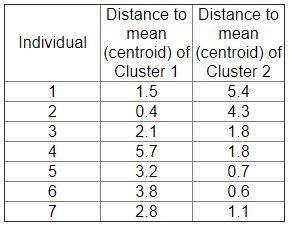
\includegraphics[scale=0.9]{kmeans_5}
	\caption{Euclidean Distance Cluster 1, Cluster 2}
	\label{fig:kmeans_5}
\end{figure}

\item Dapat disimpulkan bahwa, hanya individu 3 yang jaraknya lebih dekat dengan \textit{centroid Cluster 2} dari pada \textit{centroid Cluster 1}. Dengan kata lain, distance masing-masing individu ke \textit{centroid} kelompoknya sendiri harus lebih kecil daripada rata-rata kelompok lain. Dengan demikian, individu 3 harus dialokasikan ke \textit{Cluster 2}. Gambar \ref{fig:kmeans_6} adalah hasil pengelompokan akhir yang dihasilkan oleh pemodelan \textit{k-means}.

\begin{figure}[H]
	\centering
	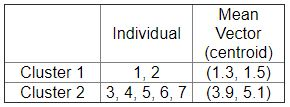
\includegraphics[scale=0.9]{kmeans_6}
	\caption{Hasil Pengelompokan Akhir}
	\label{fig:kmeans_6}
\end{figure}

\end{enumerate}
		
\newpage
		\item \textbf{Melakukan studi literatur mengenai algoritma Greedy k-member clustering}\\
		{\bf Status :} Ada sejak rencana kerja skripsi.\\
		{\bf Hasil :} Penelitian menunjukkan bahwa sebagian besar metode \textit{k-anonymity} didasarkan pada generalisasi dan teknik penekanan sehingga menderita dari kehilangan informasi yang signifikan. Masalah pengelompokan dapat meminimalkan kehilangan informasi melalui algoritma \textit{k-member clustering}. Akan tetapi algoritma \textit{k-member clustering} berpotensi memiliki kompleksitas yang eksponensial. Untuk menurunkan kompleksitas tersebut, maka permasalahan algoritma \textit{k-member clustering} dapat didefinisikan sebagai permasalahan algoritma \textit{Greedy}. Algoritma \textit{Greedy k-Member clustering} bertujuan untuk membagi seluruh data pada dataset ke masing-masing \textit{cluster} dengan kompleksitas yang lebih baik dan mendukung informasi yang lebih banyak dibandingkan algoritma \textit{clustering} yang lain.

\begin{theorem}
Masalah pengambilan keputusan pada \textit{k-member clustering} adalah \textit{NP-Hard}, artinya memiliki kompleksitas yang eksponensial.
\end{theorem}

\begin{proof}
Melalui pengamatan Aggarwal et al, permasalahan \textit{k-member clustering} dapat diselesaikan dengan kompleksitas polinomial.
\end{proof}

\begin{theorem}
$N$ adalah total data dan $k$ adalah parameter untuk anonimisasi. Setiap \textit{cluster} yang ditemukan oleh algoritma \textit{Greedy k-member clustering} memiliki jumlah tuple minimal sebanyak $k$, dan jumlah tuple tidak melebihi $2k-1$.
\end{theorem}

\begin{proof}
$S$ adalah himpunan data. Algoritma ini menemukan \textit{cluster} selama jumlah data yang tersisa sama dengan atau lebih besar dari $k$, setiap \textit{cluster} berisi $k$ data. Jika total data pada $S$ kurang dari $k$, maka sisa data akan dikelompokan pada  \textit{cluster} yang sudah ada. Oleh karena itu, ukuran maksimum sebuah \textit{cluster} adalah $2k-1$.
\end{proof}

\begin{theorem}
$N$ adalah jumlah data dan $k$ menjadi parameter anonimisasi yang ditentukan. Jika $n > k$, kompleksitas algoritma \textit{Greedy k-member clustering} adalah $O(n^2)$.
\end{theorem}

\begin{proof}
Algoritma \textit{Greedy k-member clustering} menghabiskan sebagian besar waktunya untuk memilih data dari S satu per satu hingga mencapai $|S| = k$. Karena ukuran set input berkurang satu pada setiap iterasi, total waktu eksekusi adalah O $(n^2)$.
\end{proof}

\noindent Beberapa hal penting terkait algoritma \textit{Greedy k-means clustering}:

\begin{itemize}
\item Menetapkan tabel $S$  
\item Menetapkan nilai $k$
\item Menetapkan jumlah \textit{cluster} ($m$) yang ingin dibuat
\begin{align}
m = \left \lfloor \frac{n}{k} \right \rfloor - 1
\end{align}
\end{itemize}


\noindent Berikut adalah langkah kerja algoritma \textit{Greedy k-means clustering} secara lengkap:

\begin{enumerate}
\item Melakukan inisialisasi variabel result dengan himpunan kosong dan variabel $r$ dengan memilih data secara acak dari tabel $S$

\item Pada kondisi $|S| \geq k$, lakukan perulangan sebagai berikut:

\begin{enumerate}
\item Memilih data baru pada variabel $r$ berdasarkan perbedaaan distance tertinggi dari nilai $r$ sebelumnya. Perbedaan distance dapat dicari menggunakan rumus berikut:
\begin{align*}
\Delta (r_1,r_2) = \sum_{i=1}^{m} \delta_N(r_1[N_i],r_2	[N_i]) +  \sum_{j=1}^{n} \delta_C(r_1[C_j],r_2[C_j])
\end{align*}

\noindent Berikut adalah rumus menghitung distance antar data numerik:
\begin{align*}
\delta_n(v_1,v_2) = \frac{|v_1 - v_2|}{|D|} 
\end{align*}

\vspace{0.4cm}

\noindent Berikut adalah rumus menghitung distance antar data kategorikal:

\begin{align*}
\delta_C(v_1,v_2) = \frac{H(\Lambda(v_i,v_j))}{H(T_D)} 
\end{align*}

\vspace{0.4cm}

\item Membuang himpunan data variabel $r$ pada variabel $S$

\item Mengisi data dari variabel $r$ pada variabel $c$.

\item Pada kondisi $|c| \geq k$, lakukan perulangan sebagai berikut:

\begin{enumerate}
\item Memilih data baru terbaik untuk variabel $r$ berdasarkan nilai \textit{Information Loss} (IL) yang paling rendah. \textit{Information Loss} (IL) dapat dicari menggunakan rumus berikut:

\begin{align*}
IL(e)&= |e| \cdot D(e) \\
D(e) &= \sum_{i=1}^{m} \frac{(MAX_{N_i} - MIN_{N_i})}{|N_i|} + \sum_{j=1}^{n}\frac{H(\Lambda(\cup_{C_j}))}{H(T_{C_j})}
\end{align*}

\item Membuang himpunan data dari variabel $r$ pada variabel $S$

\item Menambahkan himpunan data dari variabel $r$ pada variabel $c$.

\item Menambahkan himpunan data dari variabel $c$ pada variabel $result$

\end{enumerate}

\end{enumerate}

\item Pada kondisi $|S| \neq  0$, artinya jika masih terdapat data yang belum dimasukkan pada sebuah \textit{cluster} dari tabel $S$, lakukan perulangan sebagai berikut:

\begin{enumerate}
\item Memilih data secara acak dari tabel $S$ untuk disimpan pada variabel $r$.

\item Membuang himpunan data dari variabel $r$ pada variabel $S$.

\item Memilih \textit{cluster} terbaik untuk variabel $c$ berdasarkan nilai \textit{Information Loss} (IL) yang paling rendah. \textit{Information Loss} (IL) dapat dicari menggunakan rumus berikut:

\begin{align*}
IL(e)&= |e| \cdot D(e) \\
D(e) &= \sum_{i=1}^{m} \frac{(MAX_{N_i} - MIN_{N_i})}{|N_i|} + \sum_{j=1}^{n}\frac{H(\Lambda(\cup_{C_j}))}{H(T_{C_j})}
\end{align*}

\item Menambahkan himpunan data dari variabel $r$ pada variabel $c$.

\end{enumerate}

\item Algoritma ini mengembalikan himpunan data berdasarkan jenis \textit{cluster} yang berbeda-beda melalui variabel \textit{result}.

\end{enumerate}

\noindent Berikut adalah pseudocode secara lengkap dari algoritma \textit{Greedy k-member clustering}:
\begin{tcolorbox}[blanker,width=(\linewidth-0.5cm)]
\begin{algorithm}[H]
  \caption{Find Best Record}\label{alg:1}
  \begin{algorithmic}[1]
  %-------------- Input & Output -----------------
  \State \textbf{Function} \texttt{find\_best\_record(S,c)}
  \State \textbf{Input:} a set of records S and a cluster c.
  \State \textbf{Output:} a record r $\in$ S such that $IL(c \cup \{r\})$ is minimal
  \\
  %-------------- Baris 1-3 -----------------
  \State{$n = |S|$}
  \State{$min = \infty$}
  \State{$best = null$}
  \For{$i = 1 \ldots n$}
  \State{r = i-th record in S}
  \State{diff = $IL(c \cup \{r\}) - IL(c)$}
  \If{diff < min}
  \State{min = diff}
  \State{best = r}
  \EndIf
  \EndFor
  \State{return best}
  \end{algorithmic}
\end{algorithm}
\end{tcolorbox}

Algoritma \ref{alg:1} menerima input himpunan data dataset dan sebuah data dengan nilai \textit{distance} tertinggi dari data terpilih acak. Algoritma ini menghitung selisih \textit{distance} dari dua jenis data yang berbeda. Variabel \textit{diff} pada algoritma ini adalah perbedaan \textit{distance}, dicari dengan penjumlahan \textit{information loss} pada sebuah \textit{cluster} dengan \textit{information loss} pada data ke-i, lalu hasil penjumlahan tersebut dikurangi dengan \textit{information loss} dari \textit{kluster}. Output algoritma ini adalah sebuah data dengan nilai terbaik, yaitu data ke-i dari dataset $S$ dengan nilai \textit{distance} paling kecil.

\begin{tcolorbox}[blanker,width=(\linewidth-0.5cm)]
\begin{algorithm}[H]
  \caption{Find Best Cluster}\label{alg:2}
  \begin{algorithmic}[1]
  %-------------- Input & Output -----------------
  \State \textbf{Function} \texttt{find\_best\_cluster(C,r)}
  \State \textbf{Input:} a set of cluster C and a record r.
  \State \textbf{Output:} a cluster c $\in$ C such that $IL(c \cup \{r\})$ is minimal
  \\
  %-------------- Baris 1-3 -----------------
  \State{$n = |C|$}
  \State{$min = \infty$}
  \State{$best = null$}
  \For{$i = 1 \ldots n$}
  \State{c = i-th cluster in C}
  \State{diff = $IL(c \cup \{r\}) - IL(c)$}
  \If{diff < min}
  \State{min = diff}
  \State{best = c}
  \EndIf
  \EndFor
  \State{return best}
  \end{algorithmic}
\end{algorithm}
\end{tcolorbox}

Algoritma \ref{alg:2} menerima input himpunan data \textit{cluster} dan sebuah data dengan nilai \textit{distance} tertinggi dari data terpilih acak. Algoritma ini menghitung selisih distance dari dua jenis data yang berbeda. Variabel \textit{diff} pada algoritma ini adalah perbedaan \textit{distance}, dicari dengan penjumlahan \textit{information loss} pada sebuah \textit{cluster} dengan \textit{information loss} pada data ke-i, lalu hasil penjumlahan tersebut dikurangi dengan \textit{information loss} dari {cluster}. Output algoritma ini adalah data dengan nilai \textit{cluster} terbaik, yaitu data ke-i dari dataset S dengan nilai \textit{distance} paling kecil.

\begin{tcolorbox}[blanker,width=(\linewidth-0.5cm)]
\begin{algorithm}[H]
  \caption{Greedy K-Member Clustering}		 \label{alg:3}
  \begin{algorithmic}[1]
  %-------------- Input & Output -----------------
  \State \textbf{Function} \texttt{greedy\_k\_member\_clustering(S,k)}
  \State \textbf{Input:} a set of records S and a threshold value k
  \State \textbf{Output:} a set of clusters each of which contains at least k records.
  \\
  %-------------- Baris 1-3 -----------------
  \If{$S \leq k$} 
  \State{return S}
  \EndIf
  \\
  \State{$result = \phi$}
  \State{r = a randomly picked record from S}
  \While{$|S| \geq k$}
  \State{r = the furthest record from r}
  \State{S = S - \{r\}}
  \State{c = \{r\}}
  	\While{$|c| < k$}
	\State{r = find\_best\_record(S,c)}  
	\State{S = S - \{r\}}
  	\State{c = c $\cup$ \{r\}}
  	\EndWhile
  	\State{result = result $\cup$ \{c\}}
  \EndWhile
  \While{$S \neq 0$}
  \State{r = a randomly picked record from S}
  \State{S = S - \{r\}}
  \State{c = find\_best\_cluster(result,r)}
  \State{c = c $\cup$ \{r\}}
  \EndWhile
  \State{return result}
  \end{algorithmic}
\end{algorithm}
\end{tcolorbox}

Algoritma \ref{alg:3} menerima input himpunan data $S$ dan nilai $k$. Algoritma ini mengeksekusi dua jenis fungsi yang berbeda yaitu fungsi \textit{find\_best\_cluster} untuk mencari \textit{cluster} dengan \textit{distance} terkecil dan fungsi \textit{find\_best\_record} untuk mencari data dengan \textit{distance} terkecil. Output dari algoritma ini adalah himpunan data dari berbagai jenis \textit{cluster} dengan nilai \textit{distance} terkecil.
		
\textbf{Distance} 

\textit{Distance} adalah salah satu perhitungan untuk menyatakan akurasi terhadap utilitas sebuah data. \textit{Distance} merupakan faktor yang paling penting untuk menentukan hasil pengelompokan data. Pemilihan \textit{distance} yang baik dapat mencapai hasil klasifikasi dengan lebih optimal. Perhitungan \textit{distance} dilakukan berdasarkan pengelompokan tipe data numerik atau kategorikal. Karena masalah \textit{k-anonymity} menggunakan atribut numerik dan kategorikal, maka membutuhkan cara khusus untuk mengitung \textit{distance} dari kedua jenis data pada saat yang sama. 

\textit{Distance} data numerik direpresentasikan sebagai nilai rentang. Beberapa atribut pada \textit{distance} numerik yaitu $|D|$ adalah jumlah data pada sebuah domain berdasarkan satu atribut numerik, $v_1$, $v_2$ adalah nilai atribut numerik. \textit{Distance} data numerik dihitung menggunakan rumus berikut:

\begin{equation}
\delta_n(v_1,v_2) = \frac{|v_1 - v_2|}{|D|} 
\end{equation}

\textit{Distance} data kategorikal direpresentasikan sebagai \textit{taxonomy tree}. Beberapa atribut pada distance kategorikal yaitu $|D|$ adalah jumlah data pada domain kategorikal, $TD$ adalah \textit{taxonomy tree} untuk domain $D$,  $H(\Lambda(v_i,v_j))$ adalah jarak dari satu \textit{subtree} ke \textit{subtree} lain, $H(T_D)$ adalah tinggi dari \textit{taxonomy tree}. \textit{Distance} data kategorikal dihitung menggunakan rumus berikut:

\begin{equation}
\delta_C(v_1,v_2) = \frac{H(\Lambda(v_i,v_j))}{H(T_D)} 
\end{equation}

\textit{Distance} antar \textit{record} adalah gabungan dari \textit{distance} numerik dan kategorikal. Beberapa atribut \textit{distance} antar \textit{record} yaitu $r_1[N_i]$, $r_2[N_i]$ adalah nilai dari atribut numerik, $r_1[C_j]$, $r_2[C_j]$ adalah nilai dari atribut kategorikal, $\delta_N$ adalah \textit{distance} data numerik, $\delta_C$ adalah \textit{distance} data kategorikal. \textit{Distance} record dihitung menggunakan rumus berikut:
\begin{align}
\Delta (r_1,r_2) = \sum_{i=1}^{m} \delta_N(r_1[N_i],r_2	[N_i]) +  \sum_{j=1}^{n} \delta_C(r_1[C_j],r_2[C_j])
\end{align}


\textbf{Information Loss}

\textit{Information Loss} (IL) digunakan untuk mengevaluasi seberapa baik kinerja algoritma \textit{k-anonymity} terhadap utilitas sebuah data. Dalam menghitung \textit{Information Loss} (IL), perlu mendefinisikan beberapa atribut seperti \textit{cluster} $e = {r_1,\ldots,r_k}$  untuk \textit{quasi-identifier} yang terdiri dari atribut numerik ${N1,\ldots, Nm}$ dan atribut kategorikal ${C_1,\ldots,C_n}$, $T_{C_i}$ adalah \textit{taxonomy tree} untuk domain kategorikal $C_i$, $MIN_{N_i}$ dan $MAX_{N_i}$ adalah nilai minimum dan maksimum pada \textit{cluster} $e$ untuk atribut $N_i$, $\cup_{C_i}$ adalah sekumpulan nilai pada \textit{cluster} $e$ berdasarkan atribut $C_i$. \\

\noindent \textit{Information loss} dihitung dengan rumus sebagai berikut:
\begin{align}
IL(e)&= |e| \cdot D(e) \\
D(e) &= \sum_{i=1}^{m} \frac{(MAX_{N_i} - MIN_{N_i})}{|N_i|} + \sum_{j=1}^{n}\frac{H(\Lambda(\cup_{C_j}))}{H(T_{C_j})}
\end{align}

\noindent Total \textit{Information Loss} dihitung dengan rumus sebagai berikut:
\begin{align}
Total-IL(AT) = \sum_{e \in \varepsilon}^{}  IL(e)
\end{align}

\noindent Semakin besar total \textit{information loss} yang dihasilkan maka informasi yang dihasilkan semakin kurang akurat. Oleh karena itu perlu dilakukan beberapa eksperimen terhadap penentuan nilai $k$ pada algoritma \textit{Greedy k-member clustering} agar dihasilkan total \textit{information loss} seminimal mungkin sehingga hasil \textit{clustering} dan klasifikasi dengan nilai akurasi yang tinggi.	
		
		
		\item \textbf{Melakukan studi literatur mengenai konsep Hadoop, Spark, dan Spark MLlib}\\
		{\bf Status :} Ada sejak rencana kerja skripsi.\\
		{\bf Hasil :} Hadoop adalah \textit{framework} yang memanfaatkan beberapa komputer untuk menyelesaikan masalah yang melibatkan volume data sangat besar. Hadoop terdiri dari dua komponen penting, yaitu HDFS dan MapReduce. Kedua komponen ini saling berkaitan satu sama lain dalam pemrosesan data. Berikut adalah penjelasan singkat dari kedua komponen penting pada Hadoop:

\vspace{0.3cm}
\textbf{HDFS}

HDFS adalah sistem \textit{file} terdistribusi pada Hadoop dengan menyediakan penyimpanan data yang handal, mendukung partisi, dan toleran terhadap kesalahan pada hardware. HDFS bekerja erat dengan MapReduce dengan mendistribusikan penyimpanan dan perhitungan di seluruh \textit{cluster} dengan menggabungkan sumber daya penyimpanan yang dapat dipartisi tergantung kebutuhan. \\

\newpage
\textbf{MapReduce}

\textit{MapReduce} adalah kerangka kerja pemrosesan \textit{big data} pada sistem terdistribusi Hadoop dengan cara membagi dan memecah data yang berukuran besar menjadi blok-blok data dengan ukurang yang lebih kecil dengan memanfaatkan pemrosesan data secara paralel pada masing-masing \textit{cluster}. Pemodelan \textit{MapReduce} terdiri dari dua fungsi, yaitu \textit{Mapper} dan \textit{Reducer}. 

\begin{figure}[H]
	\centering
	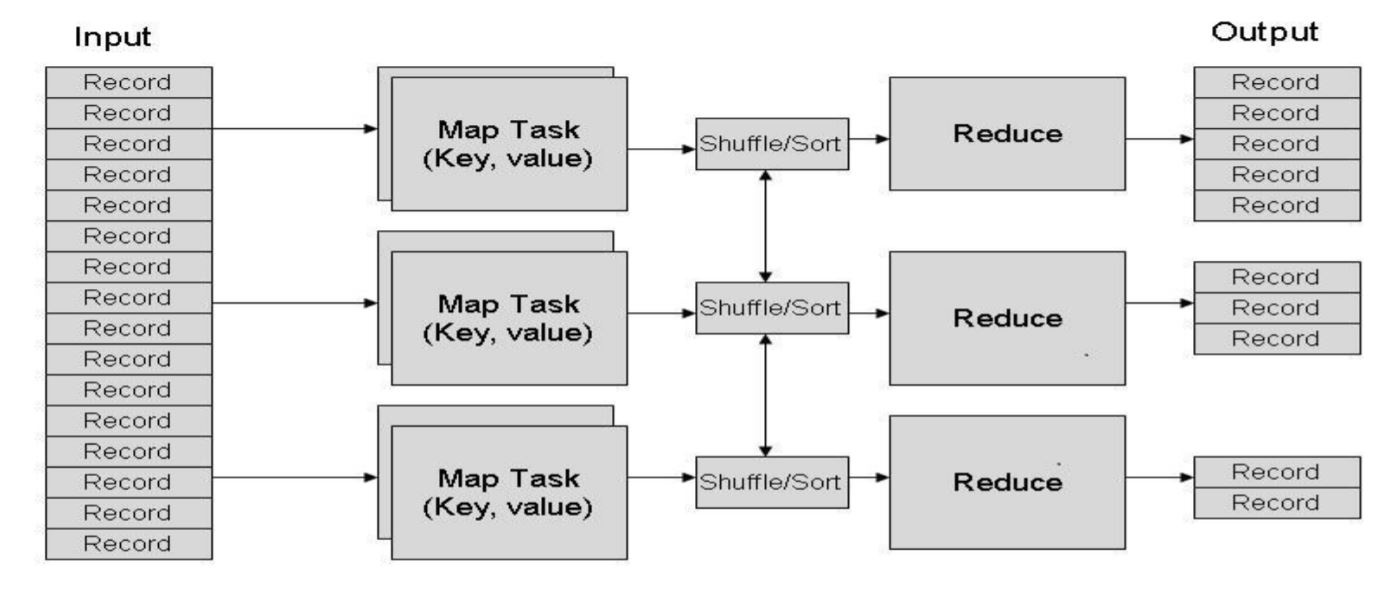
\includegraphics[scale=0.4]{MapReduceImage}
	\caption{Tahapan pada MapReduce}
	\label{fig:MapReduceImage}
\end{figure}

\noindent Gambar \ref{fig:MapReduceImage} adalah tahapan pada \textit{MapReduce}, berikut adalah penjelasannya:

\begin{itemize}
\item Input\\
Input yang diterima pada pemodelan ini adalah blok-blok data yang telah tersebar pada seluruh \textit{cluster}. Selanjutnya blok-blok data ini akan menjadi parameter input untuk fungsi \textit{Mapper} di tahap selanjutnya.

\item \textit{Mapper}\\
\textit{Mapper} memiliki fungsi untuk memetakan blok-blok data ke dalam pasangan <\textit{key},\textit{value}>. Pemetaan ini dilakukan agar pada tahap selanjutnya pasangan tersebut dapat diurutkan dan digabungkan berdasarkan nilai \textit{key}.

\item Reducer\\
\textit{Reducer} memiliki fungsi untuk mengurangi jumlah pasangan data dan membuat pasangan baru terkait jenis komputasi yang dilakukan. Berikut adalah tahapan yang dilakukan oleh \textit{Reducer}:

\begin{enumerate}

\item \textit{Shuffle} \\
\textit{Shuffle} adalah tahapan untuk pengelompokan pasangan <\textit{key},\textit{value}> pada beberapa kelompok berdasarkan nilai \textit{key} yang sama.


\item \textit{Sort} \\
Pasangan <\textit{key},\textit{value}> yang sudah dikelompokan, selanjutnya akan diurutkan. Keterurutan akan dilakukan berdasarkan nilai \textit{key}, dari terendah hingga tertinggi. 


\item \textit{Reducer} \\
Pasangan data yang sudah dikelompokan dan diurutkan, selanjutnya akan dikurangi jumlah pasangannya berdasarkan komputasi tertentu. Pasangan <\textit{key},  \textit{(list of value)}> baru akan dihasilkan pada tahap ini dan dikembalikan sebagai output.
\end{enumerate}

\item Output\\
Output yang dihasilkan adalah pasangan <\textit{key}, \textit{(list of value)}> baru berdasarkan jenis komputasi tertentu. Output ini akan dikumpulkan terlebih dahulu pada komputer \textit{master}. Selanjutnya, output ini akan ditulis ke sebuah \textit{file} oleh Reducer.
\end{itemize}
	
\newpage	
\textbf{Spark}

Spark adalah teknologi komputasi \textit{cluster} yang dirancang untuk komputasi cepat. Spark adalah paradigma pemrosesan data berukuran besar yang dikembangkan oleh para peneliti \textit{University of California} di \textit{Berkeley}. Spark adalah alternatif dari Hadoop MapReduce untuk mengatasi keterbatasan pemrosesan input output yang tidak efisien pada \textit{disk}, dengan menggunakan memori. Fitur utama Spark adalah melakukan komputasi di dalam memori sehingga waktu komputasi menjadi lebih singkat dibandingkan waktu komputasi di dalam \textit{disk}.
\\\\
Berikut adalah karakteristik dari Spark:
\begin{itemize}
\item Kecepatan\\
Spark adalah alat komputasi \textit{cluster} tujuan umum. Ini menjalankan aplikasi hingga 100 kali lebih cepat dalam memori dan 10 kali lebih cepat pada \textit{disk} daripada Hadoop. Spark mengurangi jumlah operasi baca/tulis pada \textit{disk} dan menyimpan data dalam memori.


\item Mudah untuk diatur\\	
Spark dapat melakukan pemrosesan \textit{batch}, analisis data secara interaktif, \textit{machine learning}, dan \textit{streaming} data. Semuanya pemrosesan tersebut dikerjakan pada satu komputer yang sama. Fungsi ini menjadikan Spark sebagai mesin analisis data yang lengkap. 


\item Analisis secara real-time\\
Spark dapat dengan mudah memproses data \textit{real-time}, misalnya \textit{streaming} data secara \textit{real-time} untuk ribuan peristiwa/detik. Contoh dari sumber \textit{streaming} data adalah Twitter, Facebook, Instagram. \textit{Streaming} data dapat diproses secara efisien oleh Spark.
\end{itemize}

\textbf{Ekosistem Spark}
\begin{figure}[H]
	\centering
	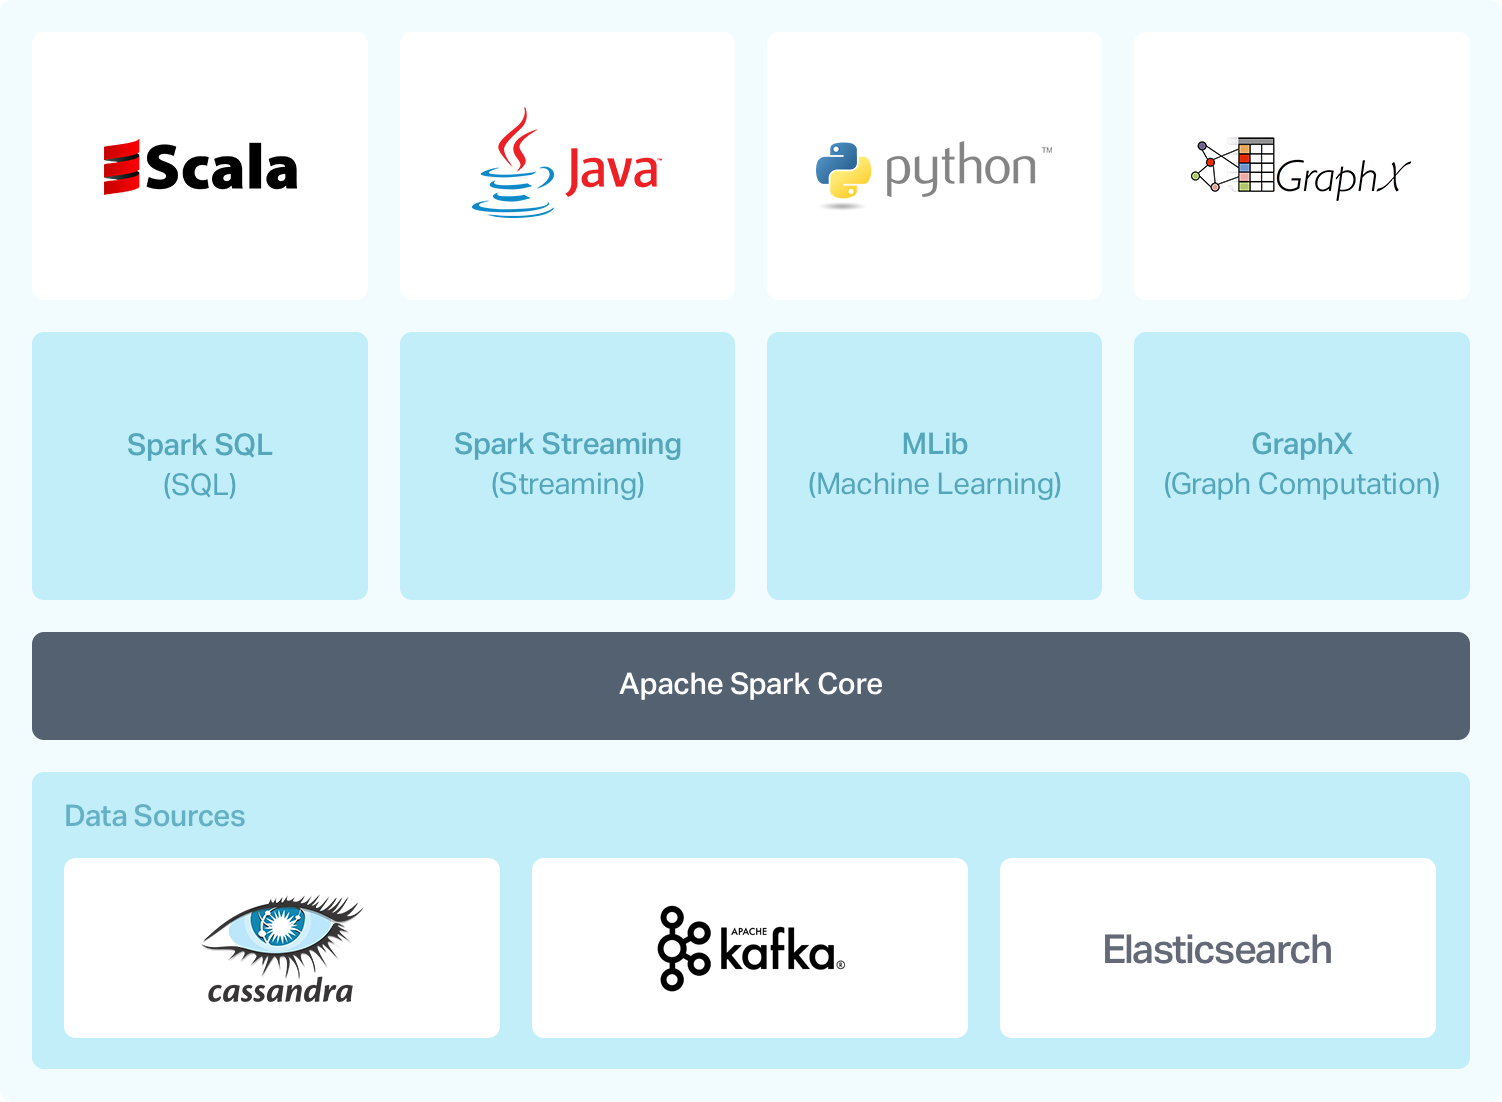
\includegraphics[scale=0.18]{spark_ecosystem}
	\caption{Ekosistem Spark}
	\label{fig:spark_ecosystem}
\end{figure}
Gambar \ref{fig:spark_ecosystem} menunjukan bahwa Spark bekerja sama dengan teknologi \textit{big data} lain untuk memenuhi berbagai macam kebutuhan dalam pengolahan \textit{big data}. Masing-masing warna pada Gambar \ref{fig:spark_ecosystem} mewakili jenis teknologi yang dipakai pada Spark. Spark SQL, Spark Streaming, Spark MLlib adalah library tambahan pada Spark. Cassandra, Kafka, dan ElasticSearch adalah \textit{framework} untuk melakukan pengumpulan data secara \textit{streaming}. Sedangkan Scala, Java, dan Python adalah bahasa pemrograman yang dapat digunakan pada Spark.

\newpage
\textbf{Arsitektur Spark}

\begin{figure}[H]
	\centering
	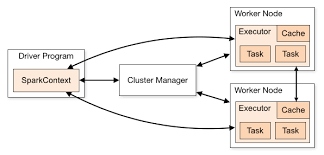
\includegraphics[scale=0.78]{arsitektur_spark2}
	\caption{Arsitektur Spark}
	\label{fig:arsitektur_spark2}
\end{figure}
Berdasarkan Gambar \ref{fig:arsitektur_spark2}, berikut adalah tahapan kerja pada arsitektur Spark:

\begin{enumerate}

\item
\textit{Program Driver} membuat \textit{Spark Context}. \textit{Spark Context} bertugas memberikan pekerjaan kepada \textit{Cluster Manager}. \textit{Spark Context} juga mencatat histori pekerjaan yang dilakukan oleh masing-masing \textit{Worker Node}, termasuk pesan error.

\item
\textit{Cluster Manager} menerima pekerjaan dari \textit{Spark Context} dan memecah pekerjaan tersebut menjadi beberapa blok data untuk diberikan kepada masing-masing \textit{Worker Node} yang aktif.

\item
\textit{Worker Node} menjalankan tugas yang diberikan oleh \textit{Cluster Manager} dan mengembalikannya ke \textit{SparkContext}. \textit{Worker Node} bertanggung jawab untuk mengerjakan tugas yang diberikan. 

\end{enumerate}

\vspace{0.2cm}
\textbf{Jenis Instalasi Spark}

\begin{figure}[H]
	\centering
	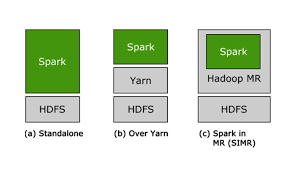
\includegraphics[scale=0.78]{arsitektur_spark}
	\caption{Arsitektur Spark}
	\label{fig:arsitektur_spark}
\end{figure}

Berdasarkan Gambar \ref{fig:arsitektur_spark}, berikut adalah jenis-jenis instalasi pada Spark:

\begin{itemize}
\item \textit{Standalone}\\  
Spark berdiri diatas HDFS Hadoop. Spark memungkinkan untuk mengakses data pada HDFS Hadoop untuk membaca input dan menulis output.

\item \textit{Hadoop Yarn}\\
Spark dapat berjalan pada Hadoop Yarn tanpa memerlukan instalasi atau meminta hak akses root apapun. Hadoop Yarn membantu integrasi Spark pada ekosistem Hadoop.

\item \textit{Spark In MapReduce} (SIMR)\\ 
SIMR digunakan untuk menjalankan pekerjaan Spark secara independen. Jenis instalasi ini sudah tidak lagi berlaku untuk Spark versi 2.0
\end{itemize}

\newpage
\textbf{Spark MLlib}

Spark MLlib adalah library pembelajaran mesin berdasarkan komputasi secara paralel. MLlib terdiri dari algoritma pembelajaran umum seperti klasifikasi, pengelompokan/\textit{clustering}. Secara garis besar, MLlib melakukan \textit{data preprocessing}, pelatihan model, dan membuat prediksi.\\

\textbf{Machine Learning pada Spark MLlib}

\begin{figure}[H]
	\centering
	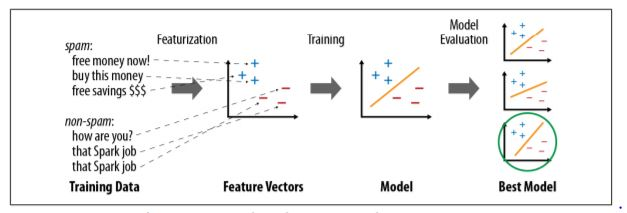
\includegraphics[scale=1]{machinelearningmllib}
	\caption{Tahapan Pembelajaran Machine Learning}
	\label{fig:machinelearningmllib}
\end{figure}
\textit{Machine learning} bertujuan membuat prediksi label/kelompok data berdasarkan jenis pemodelan \textit{data mining}. Pemodelan \textit{machine learning} membutuhkan input berupa vektor fitur. Vektor fitur adalah nilai masing-masing atribut yang digunakan pada pelatihan data. \\

\noindent Gambar \ref{fig:machinelearningmllib} adalah tahapan \textit{machine learnin}g pada Spark MLlib, berikut adalah penjelasan singkat dari masing-masing tahapan:

\begin{enumerate}

\item \textit{Featurization}\\
Pemodelan machine learning hanya dapat menerima input berupa vektor. Oleh karena itu, nilai atribut pada tabel akan diubah ke representasi numerik dalam bentuk vektor. 
 
\item \textit{Training}\\
Pemodelan machine learning melakukan pelatihan agar model yang dipakai memberikan hasil yang tepat untuk menentukan label atau kelompok data. Oleh karena itu, pemodelan machine memerlukan pelatihan model beberapa kali untuk mendapatkan model terbaik.

\item \textit{Model Evaluation}\\
Pada akhir pelatihan, model yang terbentuk dapat diputuskan baik atau tidak melalui perhitungan nilai akurasi. Semakin besar nilai akurasi, maka model dapat digunakan untuk memprediksi nilai label atau kelompok data secara tepat.
\end{enumerate}

\textbf{Data Mining pada Spark MLlib}

Data mining pada Spark MLlib menggunakan tahapan pemodelan pada \textit{machine learning} yang dijelaskan pada bagian sebelumnya untuk menghasilkan tabel hasil pengelompokan dan klasifikasi. Pada bagian ini akan dijelaskan parameter dari pemodelan Spark MLlib. Berikut adalah jenis pemodelan pada Spark MLlib:

\begin{enumerate}

\item \textit{Naive Bayes}

\textit{Naive Bayes} menjadi pemodelan klasifikasi yang umum digunakan. \textit{Naive Bayes} dapat dilatih dengan sangat efisien karena prosesnya hanya menghitung probabilitas bersyarat masing-masing atribut dan mencari probabilitas tertinggi. \textit{Naive Bayes} memiliki parameter sebagai berikut:
 
\begin{itemize}
\item \textit{randomSplit} adalah membagi \textit{training} dan \textit{test} data berdasarkan persentase.
\item \textit{setModelType} adalah memilih model yang tersedia (\textit{multinomial/bernoulli})
\item \textit{setLabelCol} adalah memilih jenis atribut yang menjadi label kelas.
\end{itemize}

\item \textit{K-Means}

\textit{K-means} menjadi pemodelan pengelompokan/\textit{clustering} yang paling umum digunakan untuk mengelompokkan titik-titik data menjadi sejumlah kelompok yang telah ditentukan. \textit{K-means} memiliki parameter masukan sebagai berikut:

\begin{itemize}
\item \textit{k} adalah jumlah \textit{cluster} yang diinginkan. 
\item \textit{maxIterations} adalah jumlah iterasi maksimum yang harus dijalankan.
\item \textit{initializationMode} menentukan inisialisasi centroid secara acak.
\item \textit{initializationSteps} menentukan jumlah langkah dalam pemodelan \textit{k-means}.
\item \textit{initialModel} adalah menentukan nilai \textit{centroid} saat dilakukan inisialisasi.
\end{itemize}

\end{enumerate}

\textbf{Tipe Data pada Spark MLlib}

Seperti yang sudah dijelaskan pada bagian sebelumnya, pemodelan \textit{machine learning} menerima input berupa vektor fitur. Tipe data yang disediakan pada Spark MLlib terdiri dari beberapa jenis yaitu vektor, \textit{labeledpoint}, dan \textit{various model class}. \\

\noindent Berikut adalah penjelasan jenis tipe data pada Spark MLlib:

\begin{itemize}
\item Vektor\\
Vektor terdiri dari dua jenis yaitu vektor \textit{dense} dan vektor \textit{sparse}. Kelas vektor berada pada \textit{package} mllib.linalg.Vectors. Gambar \ref{fig:vektor} adalah contoh vektor \textit{dense} dan vektor \textit{sparse}:

\begin{figure}[H]
	\centering
	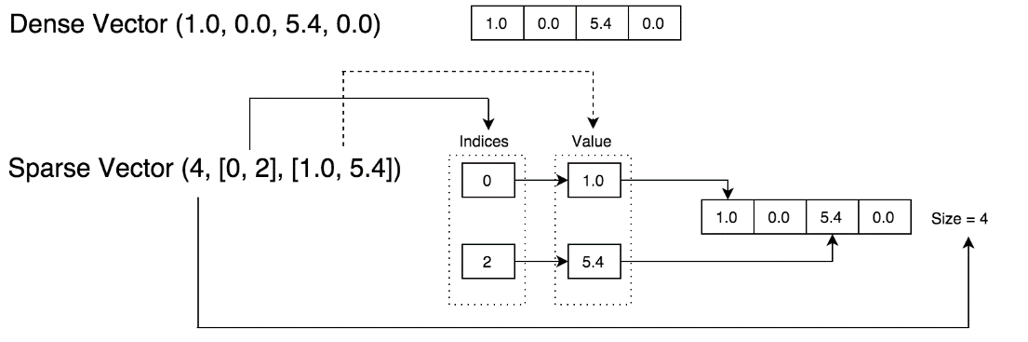
\includegraphics[scale=0.5]{vektor}
	\caption{Contoh Vektor Dense dan Sparse}
	\label{fig:vektor}
\end{figure}

\begin{itemize}

\item Vektor \textit{dense}\\
Vektor \textit{dense} adalah vektor yang menyimpan setiap nilai fitur dataset. Jumlah elemen pada vektor \textit{dense} akan memiliki jumlah yang sama dengan jumlah fitur pada dataset.

\item Vektor sparse\\
Vektor \textit{sparse} adalah vektor yang menyimpan setiap nilai fitur yang bukan nol pada dataset, sehingga jumlah elemen yang disimpan pada vektor \textit{sparse} lebih sedikit dibandingkan dengan jumlah elemen yang disimpan pada vektor \textit{dense}. 

\end{itemize}

\item \textit{LabeledPoint}\\
\textit{LabeledPoint} digunakan pada algoritma \textit{supervised learning} yaitu klasifikasi dan regresi. Kelas \textit{LabeledPoint} terletak pada \textit{package} mllib.regress.

\item \textit{Various Model class}\\
\textit{Various Model classes} adalah tipe data yang dihasilkan dari pemodelan \textit{machine learning}. Tipe data ini memiliki fungsi predict() untuk melakukan prediksi label dan kelompok data.

\end{itemize}



\item \textbf{Melakukan instalasi dan konfigurasi Spark pada cluster Hadoop}\\
		{\bf Status :} Ada sejak rencana kerja skripsi.\\
		{\bf Hasil :} Spark berjalan pada sistem operasi Windows, Linux, dan Mac OS. Spark dapat dijalankan secara lokal menggunakan satu komputer, meskipun Spark tetap membutuhkan beberapa komputer untuk pemrosesan data yang besar. Jenis instalasi Spark dijelaskan pada bagian \ref{sec:instalasi_spark}. Pada penelitian ini digunakan jenis instalasi Standalone untuk Spark versi 2.4.5 pada sistem operasi Windows. Sebelum melakukan instalasi Spark, ada beberapa hal yang harus diperhatikan dan dipenuhi.\\

\noindent Berikut adalah beberapa hal yang harus diperhatikan:

\begin{itemize}
\item Java 7, Python 2.6 telah dihilangkan pada implementasi Spark 2.2.0 ke atas.
\item Scala 2.10 sudah usang apabila dipakai pada Spark 2.4.1 ke atas.
\item Hadoop 2.6.5 telah dihilangkan pada implementasi Spark 2.2.0 ke atas.
\end{itemize}

\noindent Berikut adalah beberapa hal yang harus dipenuhi:

\begin{itemize}
\item Spark 2.4.5 dapat berjalan di Java 8, Python 2.7+/3.4+ dan R 3.1+ 
\item Spark 2.4.5 dapat menggunakan Scala 2.12
\item Spark 2.4.5 dapat menggunakan Hadoop 2.7
\end{itemize}

\noindent Berikut adalah tahapan instalasi Spark 2.4.5 secara umum:

\begin{enumerate}
\item Melakukan instalasi Java 8.
\item Melakukan instalasi Spark 2.4.5
\item Melakukan instalasi IntelIJ untuk Scala sbt.
\end{enumerate}

\textbf{Instalasi Java 8}

\noindent Berikut adalah tahapan instalasi Java 8 secara lengkap:

\begin{enumerate}

\item Download Java SE Development Kit 8u31 pada link berikut \\
\textsf{https://www.oracle.com/technetwork/java/javase/downloads/java-archive-javase8-2177648.html}
 
\item Lakukan instalasi Java SE Development Kit 8u31 seperti biasa.

\item Pilih menu \textit{Edit the system environment variables}.

\item Buat \textit{environment variables} baru seperti Gambar \ref{fig:instal_java_5}.

\begin{figure}[H]
	\centering
	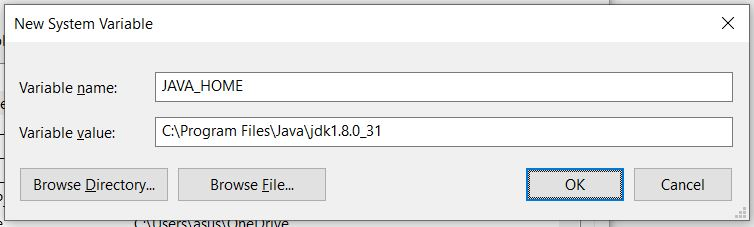
\includegraphics[scale=0.85]{instal_java_5}
	\caption{Environment Variables}
	\label{fig:instal_java_5}
\end{figure}

\newpage
\item Tambahkan \textsf{\%JAVA\_HOME\%\textbackslash bin} pada Path di \textit{System variables} seperti Gambar \ref{fig:spark_instal_5}.

\begin{figure}[H]
	\centering
	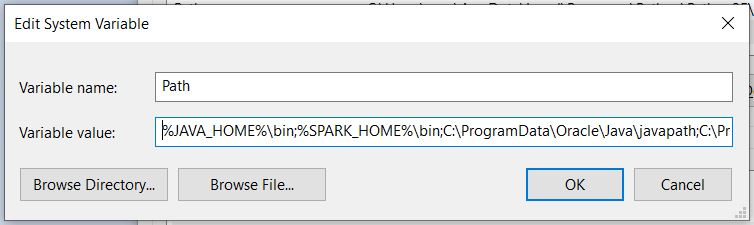
\includegraphics[scale=0.8]{spark_instal_5}
	\caption{Penambahan Variable Value}
	\label{fig:spark_instal_5}
\end{figure}


\end{enumerate}

\noindent Berikut adalah tahapan verifikasi terhadap instalasi Java 8:

\begin{enumerate}

\item Pilih menu Command Prompt.

\item Jalankan perintah java -version pada \textit{command prompt}.

\begin{figure}[H]
	\centering
	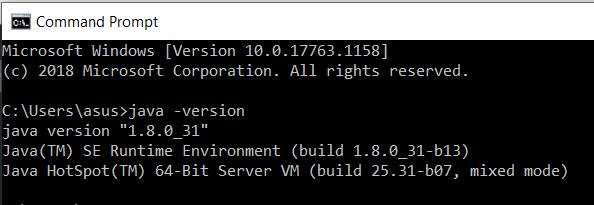
\includegraphics[scale=1]{instalasi_java}
	\caption{Perintah java -version}
	\label{fig:instalasi_java}
\end{figure}

\item Apabila sistem tidak menampilkan pesan \textit{error}, maka Java 8 sudah terpasang dengan baik.

\end{enumerate}

\textbf{Instalasi Spark 2.4.5}

Berikut adalah tahapan instalasi Spark 2.4.5 secara lengkap:

\begin{enumerate}
\item Download winutils.exe dari link \textsf{https://github.com/steveloughran/winutils/tree/master/hadoop-2.7.1/bin}, tempatkan winutils.exe pada \textsf{C:/winutils/bin}

\item Download Spark 2.4.5 dari link \textsf{https://downloads.apache.org/spark/spark-3.0.0-preview2/spark-3.0.0-preview2-bin-hadoop2.7.tgz}

\item Buat folder sebagai berikut \textsf{C:\textbackslash spark-2.4.5} dan ekstraksi \textit{file} \textsf{spark-2.4.5-bin-hadoop2.7.tgz} di dalam folder tersebut.

\item Buat \textit{environment variables} baru seperti Gambar \ref{fig:spark_instal_3}.

\begin{figure}[H]
	\centering
	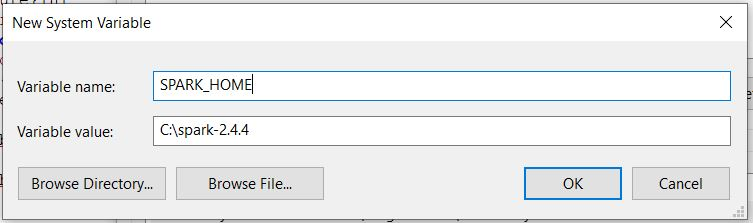
\includegraphics[scale=0.75]{spark_instal_3}
	\caption{Environment Variable}
	\label{fig:spark_instal_3}
\end{figure}

\item Tambahkan \textsf{\%SPARK\_HOME\%\textbackslash bin} pada Path di System variables sepertin Gambar \ref{fig:spark_instal_5}

\begin{figure}[H]
	\centering
	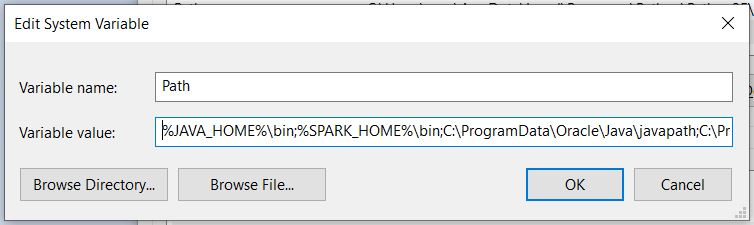
\includegraphics[scale=0.75]{spark_instal_5}
	\caption{Penambahan Variable Value}
	\label{fig:spark_instal_5}
\end{figure}

\end{enumerate}

\noindent Berikut adalah tahapan verifikasi terhadap instalasi Spark 2.4.5:
\begin{enumerate}
\item Jalankan perintah \textsf{spark-shell} pada \textit{command prompt}.

\item Apabila terminal menampilkan tampilan seperti pada Gambar \ref{fig:spark_instal_7}, artinya Spark 2.4.5 sudah dapat berjalan dengan baik pada komputer tersebut.

\begin{figure}[H]
	\centering
	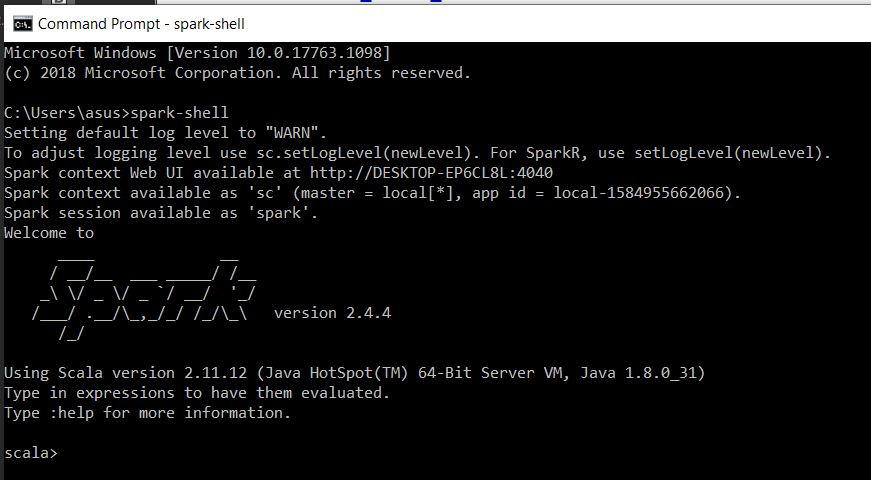
\includegraphics[scale=0.65]{spark_instal_7}
	\caption{Spark 2.4.5}
	\label{fig:spark_instal_7}
\end{figure}

\item Membuka tampilan Spark UI dengan mencantumkan alamat \textsf{localhost:4040/}  pada \textit{browser}.

\begin{figure}[H]
	\centering
	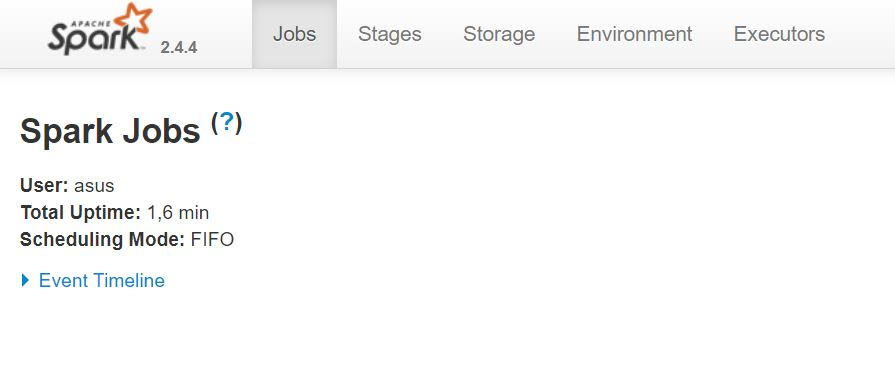
\includegraphics[scale=0.65]{spark_ui}
	\caption{Spark UI}
	\label{fig:spark_ui}
\end{figure}

\end{enumerate}

\newpage
\textbf{Instalasi IntelIJ untuk Scala SBT}

Berikut adalah tahapan instalasi IntelIJ:

\begin{enumerate}
\item Download IntelIJ melalui link berikut \\
\textsf{https://www.jetbrains.com/idea/download/\# section=windows}

\item Lakukan instalasi IntelIJ seperti biasa.
\begin{figure}[H]
	\centering
	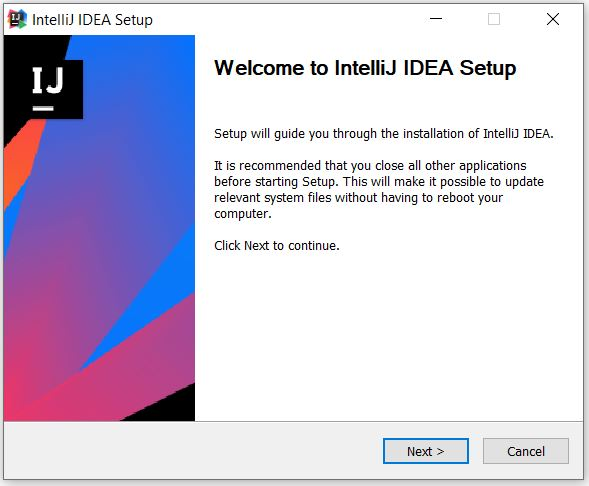
\includegraphics[scale=0.7]{intelij_install}
	\caption{Instalasi IntelIJ}
	\label{fig:intelij_install}
\end{figure}

\end{enumerate}

\noindent Berikut adalah tahapan pemasangan \textit{plugin} Scala pada IntelIJ.

\begin{enumerate}

\item Pilih menu \textit{Configure} pada IntelIJ, lalu pilih menu \textit{Plugins}.

\item Telusuri \textit{plugin} Scala pada kolom pencarian seperti Gambar \ref{fig:intelij_2}.
\begin{figure}[H]
	\centering
	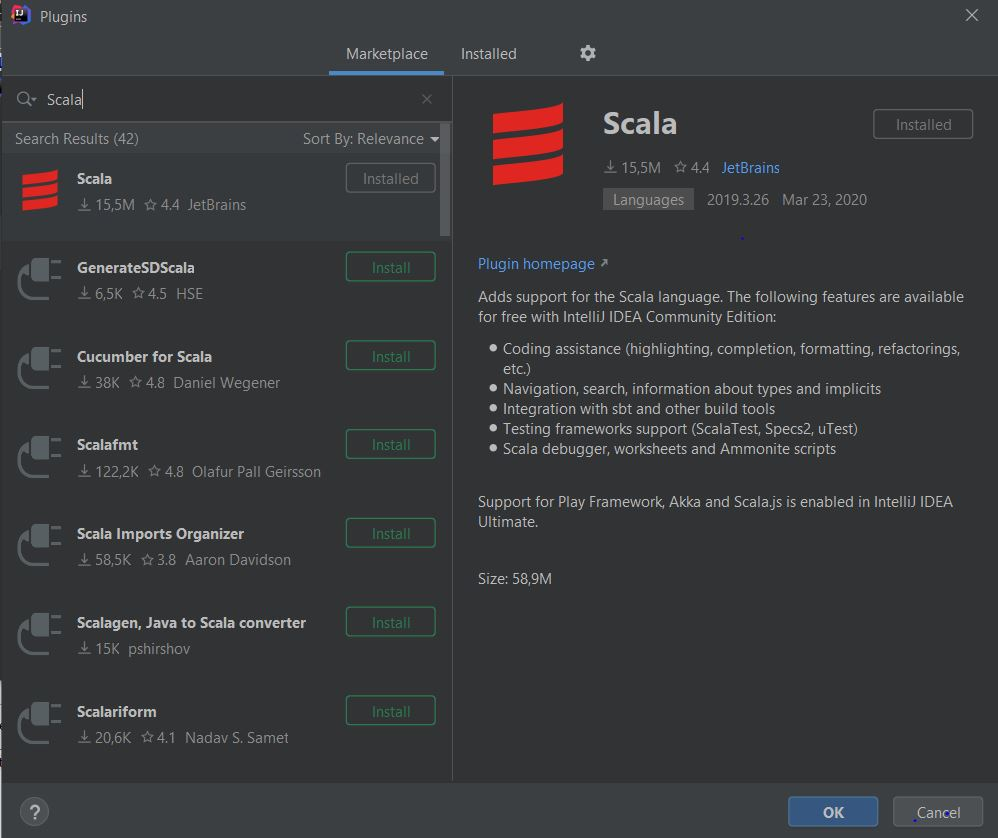
\includegraphics[scale=0.5]{intelij_2}
	\caption{Plugins Scala}
	\label{fig:intelij_2}
\end{figure}

\item Klik tombol \textit{install}

\end{enumerate}

\newpage
		\item \textbf{Melakukan studi literatur mengenai bahasa pemrograman Scala pada \textit{framework} Spark}\\
		{\bf Status :} Ada sejak rencana kerja skripsi.\\
		{\bf Hasil :} Scala adalah bahasa pemrograman berbasis \textit{open source}, dibuat oleh Profesor Martin Odersky. Scala adalah bahasa pemrograman multi-paradigma dan mendukung paradigma fungsional serta berorientasi objek. Untuk pengembangan Spark, penulisan sintaks Scala dianggap produktif untuk mengimplementasikan kode program. Pemrograman pada Scala mempertahankan prinsip keseimbangan antara produktivitas pengembangan program dan kinerja program. Pemrograman pada Scala tidak serumit pemrograman pada Java. Satu baris kode program pada Scala dapat menggantikan 20 hingga 25 baris kode Java. Karena alasan terbut, Scala menjadi bahasa pemrograman yang sangat diminati untuk melakukan pemrosesan \textit{big data} pada Spark.\\

\textbf{Scala Swing}\\
Scala Swing adalah program berbasis \textit{Graphical User Interface} (GUI) sehingga memiliki perbedaan dengan program Spark yang dieksekusi dengan terminal. Scala Swing bertujuan untuk memberi tampilan program sehingga hasil program diharapkan menjadi lebih interaktif. Scala menyediakan akses langsung terhadap kelas GUI pada Java menggunakan \textit{library} Scala Swing.  Dengan menggunakan Scala, penggunaan Scala Swing dapat memenuhi kebutuhan perancangan \textit{User Interface} melalui berbagai macam komponen GUI pada umumnya. Gambar \ref{fig:swing_example} adalah contoh implementasi GUI sederhana pada Scala Swing.

\begin{figure}[H]
	\centering
	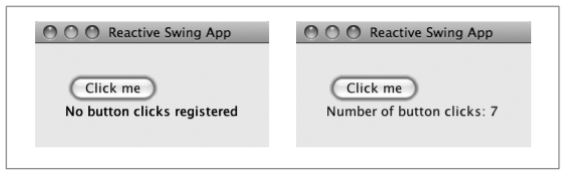
\includegraphics[scale=0.8]{swing_example}
	\caption{GUI Sederhana pada Scala Swing}
	\label{fig:swing_example}
\end{figure}

\textbf{Eksperimen Scala}

Scala digunakan pada penelitian ini karena sintaks yang sederhana untuk mengimplementasi beberapa baris kode pada bahasa pemrograman Java. Berikut adalah beberapa contoh ekperimen yang dilakukan pada bahasa Scala. Berikut adalah jenis eksperimen yang dilakukan pada Scala:

\textbf{Menentukan Jenis Variabel pada Scala}

Scala memiliki dua jenis varibel yaitu \textit{immutable} variabel dan \textit{mutable} variabel. \textit{Immutable} variabel adalah variabel yang nilainya tidak dapat diubah, sedangkan \textit{mutable} variabel adalah variabel yang nilainya dapat diubah. Implementasi \textit{immutable} dan \textit{mutable} memiliki implementasi sintaks yang berbeda. \textit{Immutable} variabel menggunakan sintaks val, sedangkan \textit{mutable} variabel menggunakan sintaks var. Kode program dapat dilihat pada Listing \ref{lst:jenis_variabel} mengenai jenis variabel pada Scala. 

\begin{lstlisting}[basicstyle=\ttfamily, frame=single,
	columns=fullflexible, keepspaces=true, breaklines=true, label=lst:jenis_variabel, caption=Menentukan Jenis Variabel pada Scala]
// Immutable Variabel
val donutsToBuy: Int = 5
donutsToBuy = 10

// Mutable Variabel
var favoriteDonut: String = "Glazed Donut"
favoriteDonut = "Vanilla Donut"


\end{lstlisting}

\textbf{Menentukan Jenis Tipe Data pada Scala}

Scala memiliki jenis tipe data yang mirip dengan tipe data pada bahasa pemrograman Java. Scala dapat menangani tipe data \textit{Int, Long, Short, Double, Float, String, Byte, Char} dan \textit{Unit}. Kode program dapat dilihat pada Listing \ref{lst:jenis_tipe_data} mengenai jenis tipe data pada Scala.

\begin{lstlisting}[basicstyle=\ttfamily, frame=single,
	columns=fullflexible, keepspaces=true, breaklines=true, label=lst:jenis_tipe_data, caption=Menentukan Jenis Tipe Data pada Scala]
val donutsBought: Int = 5
val bigNumberOfDonuts: Long = 100000000L
val smallNumberOfDonuts: Short = 1
val priceOfDonut: Double = 2.50
val donutPrice: Float = 2.50f
val donutStoreName: String = "allaboutscala Donut Store"
val donutByte: Byte = 0xa
val donutFirstLetter: Char = 'D'
val nothing: Unit = ()

\end{lstlisting}

\textbf{Menentukan Struktur Data pada Scala}

Scala memiliki dua jenis struktur data yaitu \textit{immutable} dan \textit{mutable collection}. \textit{Immutable collection} adalah struktur data yang nilainya tidak dapat diubah, sedangkan \textit{mutable collection} adalah struktur data yang nilainya dapat diubah. Implementasi \textit{immutable} dan \textit{mutable collection} memiliki jenis struktur data yang berbeda satu sama lain. Kode program dapat dilihat pada Listing \ref{lst:immutable_collection} mengenai \textit{immutable collection} pada Scala dan Listing \ref{lst:mutable_collection} mengenai \textit{mutable collection} pada Scala.

\begin{lstlisting}[basicstyle=\ttfamily, frame=single,
	columns=fullflexible, keepspaces=true, breaklines=true, label=lst:immutable_collection, caption=Membuat immutable collection pada Scala]

// List
val list1: List[String] = List("Plain Donut","Strawberry Donut","Chocolate Donut")
println(s"Elements of list1 = $list1")

// Map
val map1: Map[String, String] = Map(("PD","Plain Donut"),("SD","Strawberry Donut"),("CD","Chocolate Donut"))
println(s"Elements of map1 = $map1")
\end{lstlisting}

\begin{lstlisting}[basicstyle=\ttfamily, frame=single,
	columns=fullflexible, keepspaces=true, breaklines=true, label=lst:mutable_collection, caption=Membuat mutable collection pada Scala]
// Array
val array1: Array[String] = Array("Plain Donut","Strawberry Donut","Chocolate Donut")
println(s"Elements of array1 = ${array1.mkString(", ")}")

// Map
val map1: Map[String, String] = Map(("PD","Plain Donut"),("SD","Strawberry Donut"),("CD","Chocolate Donut"))
println(s"Elements of map1 = $map1")
\end{lstlisting}

\newpage
\textbf{Membuat Kelas Object pada Scala}

Scala menggunakan kelas \textit{Object} untuk menempatkan berbagai macam fungsi dan variabel yang saling berkaitan pada satu kelas yang sama. Kode program dapat dilihat pada Listing \ref{lst:kelas_object} mengenai kelas \textit{object} pada Scala.

\begin{lstlisting}[basicstyle=\ttfamily, frame=single,
	columns=fullflexible, keepspaces=true, breaklines=true, label=lst:kelas_object, caption=Membuat Kelas Object pada Scala]

object DonutShoppingCartCalculator {
 val discount: Double = 0.01
 def calculateTotalCost(donuts: List[String]): Double = {
  return 1
 }
}

\end{lstlisting}

\textbf{Membuat Fungsi Sederhana pada Scala}

Scala menggunakan fungsi untuk menempatkan kode program berdasarkan tujuan masing-masing. Perlu diperhatikan bahwa hasil akhir dari fungsi langsung dikembalikan tanpa memanggil perintah \textit{return}, seperti pada Java. Kode program dapat dilihat pada Listing \ref{lst:fungsi_sederhana} mengenai pembuatan fungsi pada Scala.

\begin{lstlisting}[basicstyle=\ttfamily, frame=single,
	columns=fullflexible, keepspaces=true, breaklines=true, label=lst:fungsi_sederhana, caption=Membuat Fungsi Sedehana pada Scala]

def calculateDonutCost(donutName: String, quantity: Int): Double = {
  println(s"Calculating cost for $donutName, quantity = $quantity")
  2.50 * quantity
}

\end{lstlisting}


\textbf{Membuat Main Method}

Scala menggunakan \textit{main method} untuk melakukan eksekusi program. Kode program dapat dilihat pada Listing \ref{lst:main_method} mengenai pembuatan \textit{main method} pada Scala.

\begin{lstlisting}[basicstyle=\ttfamily, frame=single,
	columns=fullflexible, keepspaces=true, breaklines=true, label=lst:main_method, caption=Membuat Main Method pada Scala]
	
object HelloWorld {
	def main(args: Array[String] {
		println("Hellow, world!")
	}
}
	
\end{lstlisting}

\textbf{Membuat Fungsi Percabangan}

Scala memiliki jenis implementasi percabangan yang sama dengan Java. Percabangan digunakan untuk melakukan eksekusi pada baris \textit{statement} yang sesuai berdasarkan kondisi tertentu. Kode program dapat dilihat pada Listing \ref{lst:percabangan} mengenai percabangan pada Scala.

\newpage
\begin{lstlisting}[basicstyle=\ttfamily, frame=single,
	columns=fullflexible, keepspaces=true, breaklines=true, label=lst:percabangan, caption=Membuat Fungsi Percabangan pada Scala]

# If-Else statement
if(numberOfPeople > 10) { 
  println(s"Number of donuts to buy = ${numberOfPeople * donutsPerPerson}")
}
else if (numberOfPeople == 0) {
  println("Number of people is zero.")
  println("No need to buy donuts.")
} 
else {
  println(s"Number of donuts to buy = $defaultDonutsToBuy")
}

\end{lstlisting}

\textbf{Membuat Fungsi Perulangan pada Scala}

Scala memiliki jenis implementasi perulangan yang sama dengan Java. Perulangan digunakan untuk mengulangi eksekusi pada baris \textit{statement} yang sama berdasarkan kondisi tertentu. Kode program dapat dilihat pada Listing \ref{lst:perulangan} mengenai perulangan pada Scala.

\begin{lstlisting}[basicstyle=\ttfamily, frame=single,
	columns=fullflexible, keepspaces=true, breaklines=true, label=lst:perulangan, caption=Membuat Fungsi Perulangan pada Scala]

# For loop
for(numberOfDonuts <- 1 to 5){
  println(s"Number of donuts to buy = $numberOfDonuts")
}

# While loop
while (numberOfDonutsToBake > 0) {
  println(s"Remaining donuts to be baked = $numberOfDonutsToBake")
  numberOfDonutsToBake -= 1
}

# Do-while loop
do {
  numberOfDonutsBaked += 1
  println(s"Number of donuts baked = $numberOfDonutsBaked")
} 
while (numberOfDonutsBaked < 5)

\end{lstlisting}
		
\vspace{0.5cm}		
		\item \textbf{Melakukan studi dan eksplorasi teknik-teknik dasar data mining pada Spark MLlib.}\\
		{\bf Status :} Ada sejak rencana kerja skripsi.\\
		{\bf Hasil :} Pada bagian sebelumnya telah dijelaskan mengenai konsep dan contoh pemodelan pada Spark MLlib. Pada penelitian ini akan digunakan pemodelan \textit{Naive Bayes} untuk permasalahan klasifikasi dan \textit{k-means} untuk permasalahan \textit{clustering}.

\newpage
\textbf{Naive Bayes}

\noindent Berikut adalah tahapan eksperimen pada Listing \ref{lst:naivebayes_mllib} untuk pemodelan \textit{Naive Bayes}:
\begin{enumerate}
\item Membagi data input CSV menjadi training data dan test data.
\item Melakukan pelatihan data pada pemodelan Naive Bayes.
\item Mengembalikan hasil klasifikasi dalam bentuk tabel.
\item Menghitung akurasi dari klasifikasi label kelas.
\end{enumerate}	

\par Hasil dari pemodelan \textit{Naive Bayes} adalah prediksi jenis \textit{cluster} berdasarkan sifat dari masing-masing data. Umumnya pada hasil pemodelan \textit{Naive Bayes} data-data yang memiliki sifat yang sama letaknya berdekatan satu sama lain. Pada Gambar \ref{fig:mllib_naivebayes}, diketahui bahwa data dengan nilai umur yang sama yaitu (\textit{age} = 17) memiliki kelompok \textit{cluster} yang sama (\textit{prediction} = 3.0).

\begin{figure}[H]
	\centering
	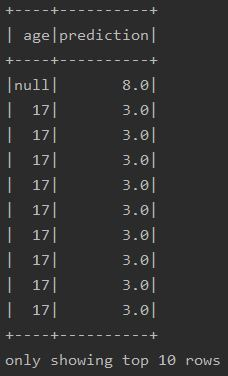
\includegraphics[scale=0.7]{mllib_naivebayes}
	\caption{Hasil Naive Bayes Spark MLlib}
	\label{fig:mllib_naivebayes}
\end{figure}

\begin{lstlisting}[basicstyle=\ttfamily, frame=single,
	columns=fullflexible, keepspaces=true, breaklines=true, label=lst:naivebayes_mllib, caption=Eksperimen Naive Bayes Spark MLlib]
// Split data into training (70%) and test (30%).
val Array(training, test) = result_df.randomSplit(Array(0.7, 0.3))

// Naive Bayes
val model = new NaiveBayes().setModelType("multinomial")
			.setLabelCol("workclass_Index").fit(training)
			
// Predict model
val predictions = model.transform(test)
predictions.show()

// Accuracy
val evaluator = new MulticlassClassificationEvaluator()
	.setLabelCol("workclass_Index")
	.setPredictionCol("prediction")
	.setMetricName("accuracy")
val accuracy = evaluator.evaluate(predictions)

\end{lstlisting}

\newpage
\textbf{K-Means}

\noindent Berikut adalah tahapan eksperimen pada Listing \ref{lst:kmeans_mllib} untuk pemodelan \textit{k-means}:
\begin{enumerate}
\item Membuat model \textit{k-means} menggunakan Spark MLlib
\item Menentukan jumlah cluster (k) untuk pemodelan \textit{k-means}.
\item Melakukan pelatihan data pada pemodelan \textit{k-means}.
\item Mencari nilai \textit{centroid} dari masing-masing \textit{cluster}.
\item Mengembalikan hasil \textit{clustering} dalam bentuk tabel.

\end{enumerate}	


\par Hasil dari pemodelan \textit{k-means} adalah prediksi jenis \textit{cluster} berdasarkan sifat dari masing-masing data. Umumnya hasil pemodelan \textit{k-means}, data-data yang memiliki perbedaan nilai atribut terkecil akan menjadi kelompok \textit{cluster} yang sama. Pada Gambar \ref{fig:mllib_kmeans}, data yang bernilai (\textit{age} = 39) memiliki kelompok \textit{cluster} yang sama (\textit{prediction} = 5) dengan data lain yang bernilai (\textit{age} = 38).

\begin{figure}[H]
	\centering
	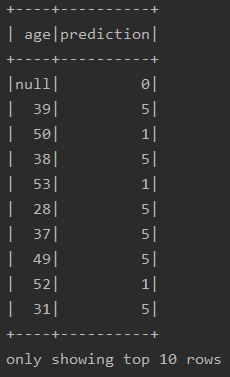
\includegraphics[scale=0.65]{mllib_kmeans}
	\caption{Hasil K-Means Spark MLlib}
	\label{fig:mllib_kmeans}
\end{figure}

\begin{lstlisting}[basicstyle=\ttfamily, frame=single,
	columns=fullflexible, keepspaces=true, breaklines=true, label=lst:kmeans_mllib, caption=Eksperimen K-Means Spark MLlib]
// KMeans with 8 clusters
val kmeans = new KMeans()
      .setK(8)
      .setFeaturesCol("features")
      .setPredictionCol("prediction")

val kmeansModel = kmeans.fit(result_df)
kmeansModel.clusterCenters.foreach(println)

// Predict model
val predictDf = kmeansModel.transform(result_df)
predictDf.show(10)
\end{lstlisting}
		
		\item \textbf{Mencari dan mengumpulkan data studi kasus}\\
		{\bf Status :} Ada sejak rencana kerja skripsi.\\
		{\bf Hasil :} Dataset yang dipakai adalah \textit{Adult}. Dataset ini diperoleh dari website Kaggle. Dataset ini disimpan dalam format CSV. Format CSV memisahkan nilai atribut data melalui simbol koma. Dataset \textit{Adult} dipilih, karena pernah digunakan sebelumnya untuk eksperimen algoritma \textit{k-anonymity}. Dataset ini berisi sampel sensus penduduk di Amerika Serikat pada tahun 1990. Penelitian ini melibatkan 10 juta baris data dengan ukuran data sebesar 1.2 GB. 

\begin{adjustwidth}{2.2cm}{0cm}
\begin{figure}[H]
	\centering
	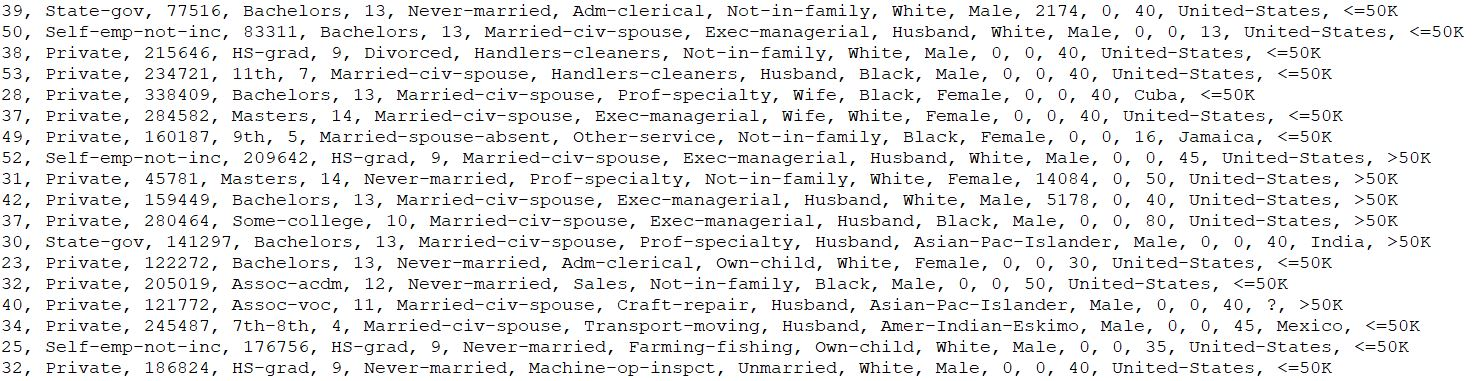
\includegraphics[scale=0.48]{dataset1}
	\caption{Dataset Adults}
	\label{fig:dataset1}
\end{figure}
\end{adjustwidth}

\noindent Berikut adalah kemungkinan nilai untuk masing-masing jenis atribut dalam dataset:

\begin{itemize}
\item Age: numerik

\item Workclass: \textit{Private, Self-emp-not-inc, Self-emp-inc, Federal-gov, Local-gov, State-gov, Without-pay, Never-worked.}

\item Education: \textit{Bachelors, Some-college, 11th, HS-grad, Prof-school, Assoc-acdm, Assoc-voc, 9th, 7th-8th, 12th, Masters, 1st-4th, 10th, Doctorate, 5th-6th, Preschool.}

\item Years of education: numerik

\item Marital status: 
\textit{Married-civ-spouse, Divorced, Never-married, Separated, Widowed, Married-spouse-absent, MarriedAF-spouse}

\item Occupation: \textit{Tech-support, Craft-repair, Other-service, Sales, Exec-managerial, Prof-specialty, Handlers-cleaners, Machine-op-inspect, Adm-clerical, Farming-fishing, Transport-moving, Priv-house-serv, Protective-serv, ArmedForces.}

\item Relationship: \textit{Wife, Own-child, Husband, Not-in-family, Other-relative, Unmarried}

\item Race: \textit{White, Asian-Pac-Islander, Amer-Indian-Eskimo, Other, Black}

\item Sex: \textit{Male, Female}

\item Capital gain: numerik

\item Capital loss: numerik

\item Hours per week: numerik

\item Native country: \textit{United-States, Cambodia, England, Puerto-Rico, Canada, Germany, Outlying-US, India, Japan, Greece, South, China, Cuba, Iran, Honduras, Philippines, Italy, Poland, Jamaica, Vietnam, Mexico, Portugal, Ireland, France, Dominican-Republic, Laos, Ecuador, Taiwan, Haiti, Columbia, Hungary, Guatemala, Nicaragua, Scotland, Thailand, Yugoslavia, El-Salvador, Trinidad and Tobago, Peru, Hong, HollandNetherlands}

\item Income: $\leq$50K, $>$50K
\end{itemize}

\textbf{Studi Kasus Personally Identifiable Information}

PII digunakan untuk mengelompokkan nilai atribut berdasarkan kategori atribut yang digunakan pada proses anonimisasi data. Berdasarkan penjelasan pada bagian sebelumnya, atribut pada proses anonimisasi dapat dikategorikan sebagai \textit{identifier, quasi-identifier}, dan \textit{sensitive attribute}. 

\par Atribut \textit{identifier} adalah atribut yang dapat mengidentifikasi individu secara langsung. Contoh dari atribut \textit{identifier} pada dataset \textit{Adult} adalah nama, tempat tanggal lahir, alamat rumah, nomor KTP. Atribut \textit{quasi-identifier} adalah atribut yang dapat mengidentifikasi seseorang apabila nilai sebuah atribut digabung dengan nilai atribut lain pada baris data yang sama. Contoh \textit{quasi-identifier} pada dataset \textit{Adult} adalah \textit{age, zip, education, years of education, occupation, race, sex, native country}. \textit{Sensitive attribute} adalah nilai yang ingin dirahasiakan. Contoh \textit{sensitive attribute} pada dataset \textit{Adult} adalah \textit{workclass, marital status, relationship, income}.

\par Atribut \textit{identifier} nantinya akan dihilangkan sebelum dilakukan proses anonimisasi, karena nilai dari atribut \textit{identifier} dapat langsung mengidentifikasi seseorang. Sedangkan \textit{sensitive attribute} nilainya tidak akan dihapus karena akan melalui proses anonimisasi bersamaan dengan nilai dari \textit{quasi-identifier} sehingga \textit{sensitive attribute} milik individu tidak dapat dibedakan satu sama lain pada hasil tabel akhir anonimisasi sehingga keamanan  distribusi data terjamin.\\

\textbf{Studi Kasus Distance, Information Loss}

Pada bagian sebelumnya, telah dijelaskan konsep mengenai penggunaan \textit{distance} dan \textit{information loss}. \textit{Distance} dan \textit{Information Loss} digunakan oleh algoritma \textit{Greedy k-member clustering} untuk mencari kelompok data terbaik sehingga menghasilkan pengelompokkan data yang tepat. Berikut adalah contoh dari masing-masing jenis perhitungan metrik:

\begin{enumerate}

\item \textit{Distance} pada Greedy k-member clustering

\textit{Distance} bertujuan untuk menentukan hasil pengelompokan data pada algoritma \textit{Greedy k-member clustering}. Pemilihan distance yang baik dapat mencapai hasil klasifikasi yang lebih optimal.
\\\\
\noindent Akan diambil 2 sampel data dari dataset \textit{Adult} sebagai berikut:
\begin{enumerate}
\item 39, State-gov, 77516, Bachelors, 13, Never-married, Adm-clerical, Not-in-family, White, Male, 2174, 0, 40, United-States, <=50K
\item 50, Self-emp-not-inc, 83311, Bachelors, 13, Married-civ-spouse, Exec-managerial, Husband, White, Male, 0, 0, 13, United-States, <=50K
\end{enumerate}

\noindent \textit{Distance} atribut numerik dapat dihitung sebagai berikut berdasarkan umur data pertama ($v_1$)= 39, umur data kedua ($v_2$)= 50, dan jumlah data ($D$)= 5 data.


\begin{align*}
\delta_n(v_1,v_2) &= \frac{|v_1 - v_2|}{|D|}
= \frac{|39 - 50|}{5}\vspace{0.2cm}
= \frac{11}{5}\vspace{0.2cm}
= 2.431
\end{align*}

\noindent \textit{Distance} atribut kategorikal dapat dihitung sebagai berikut berdasarkan \textit{workclass} data pertama ($v_1$)= \textit{State-gov, workclass} data kedua ($v_2$)= \textit{Self-emp-not-inc}, jumlah subtree ($H(\Lambda(v_i,v_j))$)= 1, dan tinggi \textit{taxonomy tree} ($H(T_D)$)= 1  seperti pada Gambar \ref{fig:TD}.

\begin{align*}
\delta_C(v_1,v_2) = \frac{H(\Lambda(v_i,v_j))}{H(T_D)} 
= \frac{1}{1}
= 1
\end{align*}

\begin{figure}[H]
	\centering
	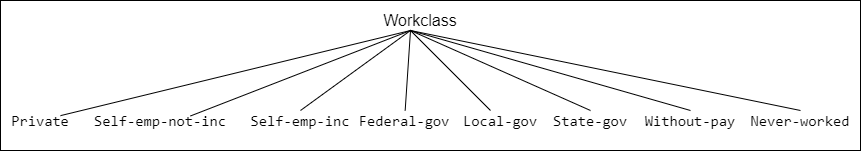
\includegraphics[scale=0.43]{TD}
	\caption{Taxonomy Tree (Workclass)}
	\label{fig:TD}
\end{figure}

\newpage
\item \textit{Information Loss} pada Greedy k-member clustering

\textit{Information Loss} (IL) bertujuan untuk mengevaluasi seberapa baik kinerja algoritma \textit{k-anonymity} terhadap utilitas sebuah data. \textit{Information Loss} (IL) juga dipakai untuk menentukan hasil pengelompokan data pada algoritma \textit{Greedy k-member clustering}. Jika diberikan tabel data yang sudah dikelompokkan berdasarkan \textit{cluster}, maka nilai \textit{Information Loss} (IL) dapat dihitung. Tabel  \ref{table:informationloss} adalah contoh hasil pengelompokan data pada \textit{cluster 1} untuk dataset \textit{Adult}:

\begin{table}[H]
\centering
\caption{Tabel Hasil Clustering Data pada Cluster 1}
\begin{adjustwidth}{1.7cm}{0cm}
\begin{tabular}{c c c c c c c c}
\hline 
Age & Workclass & Education & Occupation & Sex & Income & Cluster Name \\ 
\hline 
39 & State-gov & Bachelors & Adm-clerical & Male & <=50K & Cluster 1 \\ 
50 & Self-emp-not-inc & Bachelors & Exec-managerial & Male & <=50K & Cluster 1 \\ 
38 & Private & HS-grad & Handlers-cleaners & Male & <=50K & Cluster 1 \\ 
53 & Private & 11th & Handlers-cleaners & Male & <=50K & Cluster 1 \\ 
28 & Private & Bachelors & Prof-specialty & Female & <=50K & Cluster 1 \\ 
\hline 
\end{tabular} 
\end{adjustwidth}
\label{table:informationloss}
\end{table}

\noindent \textit{Information Loss} (IL) dapat dihitung sebagai berikut berdasarkan atribut numerik yaitu jumlah anggota \textit{cluster} ($e$)= 2, $MAX_{Age}$= 53, $MIN_{Age}$= 28, $N_Age$= 5 mencakup atribut \textit{Age} dan atribut kategorikal yaitu $H(\Lambda(\cup_{C_j}))$= 1, $H(T_{C_j})$= 1 mencakup atribut \textit{Workclass, Education, Occupation, Sex, dan Income}.

\begin{align*}
D(e) &= \sum_{i=1}^{m} \frac{(MAX_{N_i} - MIN_{N_i})}{|N_i|} + \sum_{j=1}^{n}\frac{H(\Lambda(\cup_{C_j}))}{H(T_{C_j})}\\
&= \frac{(53 - 28)}{5} + \frac{1}{1}+\frac{1}{1}+\frac{1}{1}+\frac{1}{1}+\frac{1}{1} = 10\\\\
IL(e) &= |e| \cdot D(e)\\
&= 2 \cdot 10 = 20
\end{align*}

\noindent Total \textit{Information Loss} dihitung dari jumlah \textit{Information Loss} masing-masing \textit{cluster}.

\begin{align*}
Total-IL(AT) &= \sum_{e \in \varepsilon}^{}  IL(e)\\
&= IL(cluster1)+IL(cluster2)+\ldots+IL(clusterN)
\end{align*}

\end{enumerate}
		
\textbf{Studi Kasus Algoritma Greedy k-member clustering}

Algoritma \textit{Greedy k-member clustering} telah dijelaskan pada bagian \ref{sec:greedyclustering}. Algoritma ini bertujuan untuk membagi seluruh data pada tabel terhadap masing-masing \textit{cluster} untuk kompleksitas yang lebih baik dan mendukung nilai utilitas informasi yang lebih baik dibandingkan algoritma \textit{clustering} lain. Pada bagian ini, akan dilakukan eksperimen sederhana untuk mencari tahu langkah kerja algoritma \textit{Greedy k-member clustering} secara konseptual.

\par Melalui sampel data pada Tabel \ref{table:adults}, akan diputuskan nilai dari setiap atribut anonimisasi. Jenis atribut anonimisasi yang pertama adalah Quasi-identifier, dengan nilai QI = \{\textit{Age, Education, Occupation, Sex, Income}\}. Jenis atribut anonimisasi yang kedua adalah Sensitive Attribute, dengan nilai SA = \{\textit{Workclass}\}. Jika telah diketahui tabel data seperti diatas, k = 2, dan jumlah cluster (m) = 2, maka algoritma ini siap ditelusuri lebih lanjut.

\begin{table}[H]
\centering
\caption{Dataset Adults}
\begin{tabular}{c c c c c c c c}
\hline 
ID & Age & Workclass & Education & Occupation & Sex & Income\\ 
\hline 
t1 & 39 & State-gov & Bachelors & Adm-clerical & Male & <=50K \\ 

t2 & 50 & Self-emp-not-inc & Bachelors & Exec-managerial & Male & <=50K  \\ 

t3 & 38 & Private & HS-grad & Handlers-cleaners & Male & <=50K  \\ 

t4 & 53 & Private & 11th & Handlers-cleaners & Male & <=50K  \\ 
 
t5 & 28 & Private & Bachelors & Prof-specialty & Female & <=50K	 \\ 
\hline 
\end{tabular} 
\label{table:adults}
\end{table}

\noindent Berikut adalah tahapan yang terjadi pada algoritma \textit{Greedy k-member clustering}:

\begin{enumerate}
\item Nilai awal result = $\emptyset$, $r = \{t1\}$, $|S|$ = 5, $k = 2$
\item Karena kondisi $|S| \geq k$ terpenuhi, maka dilakukan perulangan sebagai berikut:
\begin{enumerate}
\item Nilai r diubah menjadi r = \{t3\}, karena terbukti data t3 memiliki $\Delta(t1,t3)=1.7189$ yang paling tinggi dari seluruh \textit{distance} lain. Berikut adalah contoh perhitungannya:
\begin{align*}
\Delta (t_1,t_2) = 1.715\\
\Delta (t_1,t_3) = 2.431\\
\Delta (t_1,t_4) = 2.122\\
\Delta (t_1,t_5) = 1.621 
\end{align*}
\item Nilai awal $S = \{t1, t2, t4, t5\}$
\item Nilai awal $c = \{t3\}, |c| = 1$
\item Karena kondisi $|c| < k$ terpenuhi, maka dilakukan perulangan sebagai berikut:

\begin{enumerate}
\item Nilai $r$ diubah menjadi $r = \{t3,t4\}$, karena terbukti data $t4$ memiliki $IL(t3 \cup t4)=0.330$ yang paling rendah dari seluruh data lain. Berikut adalah contoh perhitungannya:
\begin{align*}
IL(t3 \cup t1) = 0.479 \\
IL(t3 \cup t2) = 0.515 \\
IL(t3 \cup t4) = 0.330 \\
IL(t3 \cup t5) = 0.367 
\end{align*}
\item Nilai $S$ diubah menjadi $S = \{t1, t2, t5\}$, $|S| = 4$
\item Nilai $c$ ditambahkan menjadi $c = \{t3, t4\}$, $|c| = 2$

\end{enumerate}
\item Karena kondisi $|c| < k$ sudah tidak terpenuhi lagi, maka perulangan ini akan berhenti
\item Nilai \textit{result} akan ditambahkan menjadi $result = \{t3, t4\}$
\item Karena kondisi $|S| \geq k$ masih terpenuhi, maka perulangan akan tetap berlanjut sampai pada kondisi dimana $|S| < k$ sehingga hasil akhirnya adalah $result = \{\{t3, t4\}, \{t2, t5\}\}$, $S = \{t1\}$, $|S| = 1$.

\end{enumerate}

\item Karena kondisi $S \neq 0$ terpenuhi, maka dilakukan perulangan sebagai berikut:

\begin{enumerate}
\item Nilai $r$ diubah menjadi $r = \{t1\}$

\item Nilai $S$ diubah menjadi S = $\{\phi\}$, |S| = 0

\item Nilai $c$ diubah menjadi c = \{t3, t4\} karena terbukti \textit{cluster} $c$ memiliki $IL(\{t3,t4\} \cup t1)=0.279$ yang paling rendah dari seluruh \textit{cluster} lain. Berikut adalah contoh perhitungannya:
\begin{align*}
IL(\{t3,t4\} \cup t1) = 0.279 \\
IL(\{t2,t5\}\cup t1) = 0.515 
\end{align*}

\item Nilai $c$ ditambahkan menjadi $c = \{t1, t3, t4\}$

\item Nilai $c$ pada perulangan ini tidak ditambahkan pada \textit{result}, karena  ditetapkan $k = 2$ sedangkan jumlah datanya ganjil, sehingga sisa data tersebut tidak akan dicatat.

\item Karena kondisi $S \neq 0$ sudah tidak terpenuhi lagi, maka perulangan ini akan berhenti.

\end{enumerate}

\item Hasil akhirnya adalah $result = \{\{t3, t4\}, \{t2, t5\}\}$ dikembalikan sebagai output untuk algoritma \textit{Greedy k-member clustering} seperti pada Tabel \ref{table:greedykmember} sebagai berikut:
\begin{table}[H]
\centering
\caption{Tabel Hasil Greedy K-Member Clustering}
\begin{tabular}{c c c c c c c c}
\hline 
ID & Age & Workclass & Education & Occupation & Sex & Income\\ 
\hline 
t3 & 38 & Private & HS-grad & Handlers-cleaners & Male & <=50K  \\ 
t4 & 53 & Private & 11th & Handlers-cleaners & Male & <=50K  \\ 
\hline 
t2 & 50 & Self-emp-not-inc & Bachelors & Exec-managerial & Male & <=50K  \\ 
t5 & 28 & Private & Bachelors & Prof-specialty & Female & <=50K	 \\ 
\hline 
\end{tabular} 
\label{table:greedykmember}
\end{table}

\end{enumerate}

\textbf{Studi Kasus Domain Generalization Hierarchy}

DGH bertujuan  melindungi data dengan menerapkan metode generalisasi terhadap nilai atribut yang unik menjadi nilai yang lebih umum. Berikut adalah penerapan DGH terhadap dataset \textit{Adult}. 

\noindent Diketahui kemungkinan nilai unik atribut pada dataset \textit{Adult} sebagai berikut:

\begin{itemize}
\item Age = \{33,36,38,40,42,43,46,49\}
\item ZIP = \{77516,77517,77526,77527\}
\item Sex = \{Male,Female\}
\end{itemize}

\noindent Untuk atribut ZIP, akan dibangun tiga jenis domain sebagai berikut:

\begin{itemize}
\item Domain dengan nilai kurang spesifik\\
Domain ini dipilih apabila tujuannya adalah lebih mengutamakan hasil informasi yang diperoleh dengan cara melakukan sedikit anonimisasi pada nilai data. Contohnya atribut ZIP akan diubah menjadi \{7751*,7752*\} apabila satu digit terakhir memiliki nilai yang berbeda dan digit sisanya memiliki nilai yang sama.

\item Domain dengan nilai yang lebih umum\\
Domain ini dipilih apabila tujuannya adalah menyeimbangkan nilai informasi yang diperoleh dengan tingkat perlindungan data yang didapat dengan cara meningkatkan level anonimisasi nilai data. Contohnya atribut ZIP akan diubah menjadi \{775**\} apabila kedua digit terakhir memiliki nilai yang berbeda dan digit sisanya memiliki nilai yang sama.

\item Domain dengan nilai yang umum.\\
Domain ini dipilih apabila tujuannya adalah mengutamakan perlindungan data. Biasanya jenis domain ini jarang dipilih, karena hasil anonimisasinya tidak dapat digunakan untuk proses data mining (memiliki nilai akurasi yang rendah apabila dilakukan pemodelan \textit{data mining}). Contohnya atribut ZIP akan diubah menjadi \{*****\}

\end{itemize}

\noindent Nilai atribut \textit{Age} akan dibangun berdasarkan ketentuan berikut: 

\begin{itemize}
\item Nilai atribut \textit{Age} akan diubah menjadi rentang nilai. Contohnya nilai 33  diubah menjadi [30-39], karena 33 termasuk pada rentang nilai tersebut.
\end{itemize}

\noindent Nilai atribut\textit{Sex} akan dibangun berdasarkan ketentuan berikut: 

\begin{itemize}
\item Nilai atribut \textit{Sex} termasuk nilai kategorikal, sehingga akan diubah menjadi nilai yang lebih umum. Contohnya nilai \textit{Male/Female} diubah menjadi \textit{Person} (bentuk umum).
\end{itemize}
		
\textbf{Studi Kasus K-Anonymity}

\textit{K-anonymity} bertujuan untuk menyamarkan nilai dari masing \textit{quasi-identifier} yang unik pada kelompok \textit{cluster} yang sama. Kata kuncinya adalah nilai unik pada kelompok \textit{cluster} yang sama. Setelah dataset dilakukan anonimisasi, maka data privasi sudah terlindungi sehingga publikasi data dapat dilakukan dengan aman. Tabel \ref{table:clustering} adalah kelompok data yang dihasilkan oleh algoritma \textit{Greedy k-member clustering}. Setelah data dikelompokan, maka data siap untuk dilakukan anonimisasi

\begin{table}[H]
\centering
\caption{Tabel Hasil Clustering}
\begin{tabular}{c c c c c c c c}
\hline 
ID & Age & Workclass & Education & ZIP & Sex & Hours/week & Cluster Name\\ 
\hline 
t3 & 32 & Private & HS-grad & 77516 & Male & 30 & Cluster 1 \\ 
t4 & 32 & Private & 11th & 77541 & Female & 30 & Cluster 1 \\ 
\hline 
t2 & 34 & Self-emp-not-inc & Bachelors & 77526 & Male & 34 & Cluster 2 \\ 
t5 & 50 & Private & Bachelors & 77526 & Male & 37	& Cluster 2\\ 
\hline 
t1 & 47 & Local-gov & Bachelors & 77581 & Male & 54 & Cluster 3\\ 
t6 & 50 & Federal-gov & HS-grad & 77532 & Male & 57 & Cluster 3\\ 
\hline 
\end{tabular} 
\label{table:clustering}
\end{table}
\vspace{0.4cm}

\noindent Diketahui bentuk generalisasi berdasarkan \textit{Domain Generalization Hierarchy} sebagai berikut:
\begin{align*}
Age &= \{[20-30], [40-50]\}\\
ZIP &= \{775**\}\\
Sex &= \{Person\}\\
Hours/week &=\{[12-18], [33-37], [53-61]\}
\end{align*} 

\noindent Berikut adalah tahapan yang terjadi pada proses anonimisasi:
\begin{enumerate}

\item Diketahui \textit{quasi-identifier} sebagai berikut QI = \{\textit{Age, ZIP, Sex, Hours/week}\} dan \textit{sensitive attribute} sebagai berikut SA = \{\textit{Workclass, Education}\}

\item Mencari nilai \textit{quasi-identifier} yang unik pada kelompok \textit{cluster} yang sama. Sebagai contoh, \textit{cluster 2} memiliki nilai \textit{quasi-identifier} yang unik sebagai berikut QI = \{\textit{Age, Hours/week}\}

\item Melakukan generalisasi DGH pada nilai \textit{quasi-identifier} yang unik menjadi bentuk generalisasi. Sebagai contoh, QI = \{\textit{Age, Hours/week}\} memiliki nilai yang unik, sehingga diubah menjadi \textit{Age} = \{[40-50]\}, \textit{Hours/week} = \{[33-37]\}

\item \textit{Sensitive attribute} tidak akan dilakukan generalisasi, karena \textit{quasi-identifier} sudah dilakukan generalisasi sehingga seseorang akan sulit untuk menebak kepemilikan dari \textit{sensitive attribute}.

\item Ulangi hal yang sama pada langkah sebelumnya untuk setiap \textit{cluster}. Hasil akhir dari proses anonimisasi ada pada Tabel \ref{table:anonimisasi} sebagai berikut: 
\begin{table}[H]
\centering
\caption{Tabel Hasil Anonimisasi}
\begin{adjustwidth}{1.7cm}{0cm}
\begin{tabular}{c c c c c c c c}
\hline 
ID & Age & Workclass & Education & ZIP & Sex & Hours/week & Cluster Name\\ 
\hline 
t3 & 32 & Private & HS-grad & 775** & Person & 30 & Cluster 1 \\ 
t4 & 32 & Private & 11th & 775** & Person & 30 & Cluster 1 \\ 
\hline 
t2 & [40-50] & Self-emp-not-inc & Bachelors & 77526 & Male & [33-37] & Cluster 2 \\ 
t5 & [40-50] & Private & Bachelors & 77526 & Male & [33-37]	& Cluster 2\\ 
\hline 
t1 & [40-50] & Local-gov & Bachelors & 775** & Male & [53-61] & Cluster 3\\ 
t6 & [40-50] & Federal-gov & HS-grad & 775** & Male & [53-61] & Cluster 3\\ 
\hline 
\end{tabular} 
\end{adjustwidth}
\label{table:anonimisasi}
\end{table}

\end{enumerate}
		
\newpage
\item \textbf{Membuat diagram kelas perangkat lunak anonimisasi}\\
		{\bf Status :} Ada sejak rencana kerja skripsi.\\
		{\bf Hasil :} Diagram kelas bertujuan untuk menggambarkan keterhubungan antar kelas. Pada penelitian ini digambarkan diagram kelas untuk perangkat lunak anonimisasi data. Karena perangkat lunak analisis data hanya memiliki satu kelas saja, maka keterhubungan antar kelas tidak perlu digambarkan dalam diagram kelas. Gambar \ref{fig:diagram_kelas} menggambarkan keterhubungan antar kelas pada perangkat lunak anonimisasi data. Berikut adalah penjelasan lengkap mengenai deskripsi kelas dan method pada perangkat lunak anonimisasi data:
		
\begin{figure}[H]
	\centering
	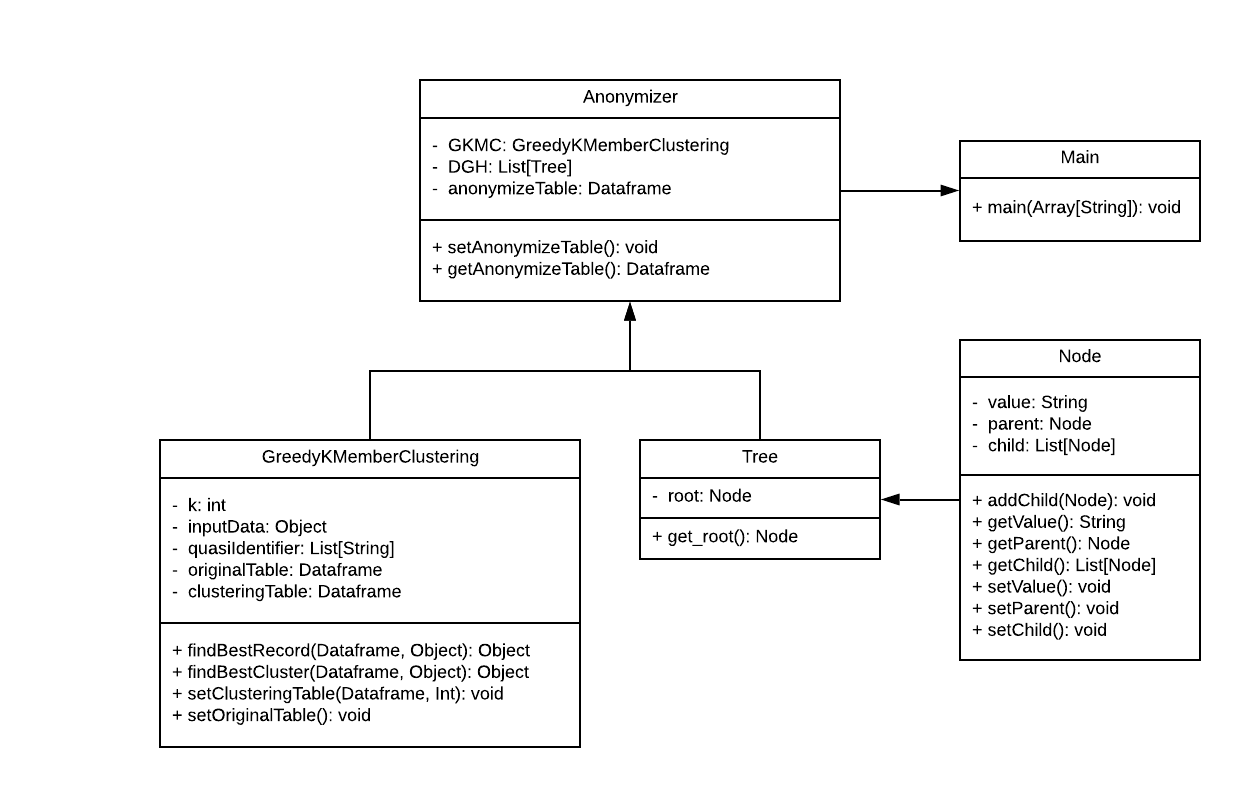
\includegraphics[scale=0.7]{diagram_kelas}
	\caption{Diagram Kelas Anonimisasi Data}
	\label{fig:diagram_kelas}
\end{figure}

\begin{itemize}
\item Kelas \textit{Anonymizer} bertujuan untuk melakukan proses anonimisasi setelah data dikelompokan menjadi beberapa \textit{cluster}. Kelas \textit{Anonymizer} memiliki 2 jenis variabel, yaitu:

\begin{itemize}

\item \textit{GKMC} adalah objek dari kelas \textit{GreedyKMemberClustering} yang berisi tabel hasil pengelompokan data berdasarkan algoritma \textit{Greedy k-member clustering}.

\item \textit{DGH} adalah array 1 dimensi dari objek \textit{Tree} yang berisi hasil anonimisasi untuk nilai quasi-identifier yang unik agar menjadi nilai yang lebih umum.

\item \textit{anonymizeTable} adalah array 2 dimensi dari kelas Object untuk menyimpan tabel hasil anonimisasi data.

\end{itemize}

\noindent Kelas \textit{Anonymizer} memiliki 2 jenis method, yaitu:

\begin{itemize}

\item \textit{setAnonymizeTable()} bertujuan untuk melakukan proses anonimisasi pada masing-masing baris data yang tergabung dalam sebuah \textit{cluster}, berdasarkan perbedaan nilai dari beberapa \textit{quasi-identifier}.

\item \textit{getAnonymizeTable()} bertujuan untuk mengambil nilai pada atribut \textit{anonymizeTable}.

\end{itemize}

\item Kelas \textit{GreedyKMemberClustering} bertujuan untuk melakukan pengelompokan data menjadi beberapa \textit{cluster} berdasarkan sifat/nilai atribut yang dimiliki oleh masing-masing baris data. Kelas \textit{GreedyKMemberClustering} memiliki 5 jenis variabel, yaitu:

\begin{itemize}

\item \textit{k} adalah variabel bertipe \textit{Integer} untuk membatasi jumlah anggota pada sebuah \textit{cluster} agar memiliki jumlah yang tetap sebanyak jumlah tertentu.

\item \textit{inputData} adalah variabel untuk menyimpan seluruh baris data \textit{file} CSV.

\item \textit{quasiIdentifier} adalah daftar dari nama-nama kolom yang akan dipilih untuk membuat tabel baru yang digunakan pada proses anonimisasi data

\item \textit{originalTable} adalah tabel yang menyimpan seluruh baris data pada file CSV berdasarkan jenis kolom yang terpilih pada variabel \textit{quasiIdentifier}.

\item \textit{clusteringTable} adalah tabel yang menyimpan hasil pengelompokan baris data dari algoritma \textit{Greedy k-member clustering}.

\end{itemize}

\noindent Kelas \textit{GreedyKMemberClustering} memiliki 4 jenis method, yaitu:

\begin{itemize}
\item \textit{findBestRecord()} bertujuan mencari sebuah baris data yang memiliki nilai \textit{information loss} yang paling minimal dengan baris data lainnya. 

\item \textit{findBestCluster()} bertujuan mencari sebuah \textit{cluster} data yang memiliki nilai \textit{information loss} yang paling minimal dengan \textit{cluster} lainnya.

\item \textit{setClusteringTable()} bertujuan mengelompokkan data berdasarkan algoritma \textit{Greedy k-member clustering} dan hasilnya disimpan pada variabel \textit{clusteringTable}.

\item \textit{setOriginalTable()} bertujuan mengubah hasil pembacaan data input CSV menjadi tabel baru dan hasilnya disimpan pada variabel \textit{originalTable}.

\end{itemize}

\item Kelas \textit{Tree} bertujuan untuk membuat pohon generalisasi berdasarkan jenis atribut \textit{quasi-identifier} yang dipilih.

\item Kelas \textit{Node} bertujuan untuk menyimpan seluruh nilai \textit{quasi-identifier} yang unik untuk masing-masing baris data.

\item Kelas \textit{Main} bertujuan untuk membuat tahapan anonimisasi dari awal sampai akhir dengan memanfaatkan pemanggilan \textit{method} dari masing-masing objek kelas.

\end{itemize}
		
		\item \textbf{Membuat diagram aktivitas perangkat lunak anonimisasi dan analisis}\\
		{\bf Status :} Ada sejak rencana kerja skripsi.\\
		{\bf Hasil :} Penelitian ini memiliki dua jenis diagram aktivitas,  yaitu diagram aktivitas untuk perangkat lunak anonimisasi data dan diagram aktivitas untuk perangkat lunak analisis data. Tujuan dari membuat dua jenis perangkat lunak antara lain untuk memisahkan perangkat lunak berdasarkan tujuan fungsionalitas yang berbeda. 

\textbf{Perangkat Lunak Anonimisasi Data}

Perangkat lunak anonimisasi adalah perangkat lunak yang digunakan untuk menyamarkan nilai data menggunakan metode anonimisasi. Perangkat lunak ini akan memiliki fungsi untuk menyamarkan beberapa nilai data agar sebuah data tidak dapat dibedakan dengan $k-1$ data lainnya berdasarkan konsep \textit{k-anonymity}. Algoritma \textit{Greedy k-member clustering} akan diimplementasikan pada Spark dengan fungsi utama yaitu menyamarkan nilai atribut data pada kelompok data yang sejenis. Berikut adalah tahapan yang terjadi pada perangkat lunak saat melakukan proses anonimisasi data:

\begin{enumerate}

\item Pengguna memberi masukan dalam format file CSV dan beberapa jenis atribut \textit{quasi-identifier} untuk menjadi tabel input pada proses anonimisasi.

\item Perangkat lunak menampilkan sebagian baris data dari tabel input karena baris data yang akan digunakan pada eksperimen akan berjumlah sangat banyak .

\item Pengguna akan meninjau ulang apakah jumlah kolom yang ditampilkan sudah sesuai dengan jumlah atribut \textit{quasi-identifier} yang akan dipakai.

\item Penggunakan memberikan parameter tambahan seperti rentang nilai k untuk menentukan jumlah anggota \textit{cluster} dan objek DGH untuk proses anonimisasi.

\item Perangkat lunak akan melakukan proses anonimisasi dengan bantuan Spark pada tabel input berdasarkan paramater tambahan yang diberikan sebelumnya. 

\item Perangkat lunak mengembalikan seluruh isi \textit{log} yang dihasilkan selama proses eksekusi Spark berlangsung kepada pengguna untuk deteksi \textit{error}.

\item Perangkat lunak hanya menampilkan baris data yang berubah akibat proses anonimisasi pada GUI dan hasil keseluruhannya dalam format \textit{file} CSV.

\item Perangkat lunak mengembalikan nilai \textit{information loss} pada masing-masing \textit{cluster} yang terbentuk agar pengguna dapat mencari hasil yang optimal.

\item Pengguna dapat membandingkan hasil anonimisasi antara baris data yang berubah akibat proses anonimisasi dengan baris data yang ada pada tabel asli.

\item Pengguna dapat mengulangi eksperimen untuk mencari nilai k terbaik agar dihasilkan \textit{information loss} seminimal mungkin pada proses anonimisasi.


 
\end{enumerate}

\textbf{Perangkat Lunak Analisis Data}

Perangkat lunak analisis data adalah perangkat lunak yang digunakan untuk melakukan pengujian \textit{data mining} pada pemodelan klasifikasi dan \textit{clustering}. Perangkat lunak ini akan memiliki fungsi untuk mencari label kelas berdasarkan pemodelan klasifikasi dan mengelompokan data berdasarkan pemodelan \textit{clustering}. Pemodelan \textit{naive bayes} dan \textit{k-means} akan diimplementasikan pada Spark dengan fungsi utama yaitu memprediksi kelompok data. Berikut adalah tahapan yang terjadi pada perangkat lunak saat melakukan pemodelan \textit{data mining}:

\begin{enumerate}

\item Pengguna memberi dua jenis masukan yaitu data asli dan data hasil anonimisasi dalam format \textit{file} CSV untuk menjadi tabel input pada proses analisis data.

\item Perangkat lunak hanya menampilkan sebagian baris data dari dua jenis tabel input karena input baris data pada eksperimen berjumlah sangat banyak 

\item Pengguna meninjau kembali apakah jumlah kolom yang ditampilkan pada kedua jenis tabel memiliki jumlah kolom atribut yang sama.

\item Pengguna memilih jenis pemodelan data mining yang tersedia pada eksperimen, yaitu klasifikasi dengan \textit{Naive Bayes} atau pengelompokan/\textit{clustering} dengan \textit{k-means}. 

\item Pengguna mengisi parameter pada pemodelan yang dipilih. Contoh pada \textit{k-means} adalah nilai k dan satu jenis atribut. Sedangkan pada \textit{Naive Bayes} adalah persentase \textit{training, testing} data dan satu jenis atribut.

\item Perangkat lunak akan melakukan proses pelatihan data pada Spark untuk menemukan klasifikasi/pengelompokan yang sesuai berdasarkan jenis pemodelan yang dipilih.

\item Perangkat lunak mengembalikan seluruh isi \textit{log} yang dihasilkan selama proses eksekusi Spark berlangsung kepada pengguna untuk deteksi \textit{error}.

\item Perangkat lunak menampilkan sebagian hasil prediksi \textit{cluster} untuk masing-masing data dan menyimpan hasil keseluruhannya dalam format \textit{file} CSV.

\item Pengguna melakukan analisis lebih lanjut terkait pengelompokan dan klasifikasi kelompok data yang terbentuk dari proses pemodelan \textit{data mining}.

\end{enumerate}

\item \textbf{Menulis dokumen skripsi}\\
		{\bf Status :} Ada sejak rencana kerja skripsi.\\
		{\bf Hasil :} Penulisan dokumen skripsi sampai saat ini masih dalam tahap pengerjaan. Penyusunan bab yang telah dibuat pada skripsi ini tersusun dari bab 1 yang berisi pendahuluan, bab 2 yang berisi dasar teori, dan bab 3 yang berisi analisis masalah. Seluruh pengerjaan dari bab 1 sampai dengan bab 3 telah selesai dikerjakan dengan baik. 

\newpage
\begin{figure}[H]
	\centering
	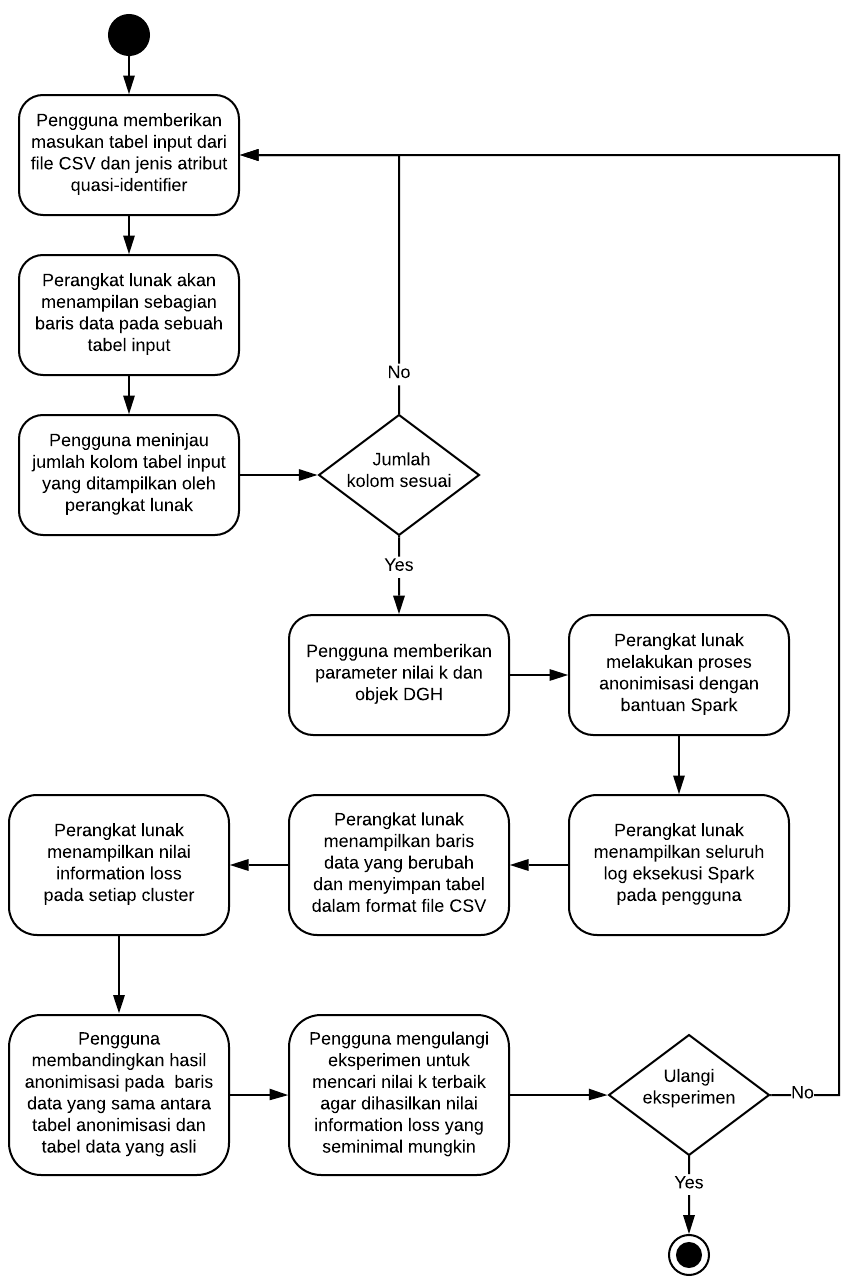
\includegraphics[scale=0.8]{pl_anonimisasi}
	\caption{Diagram Aktifitas Anonimisasi Data}
	\label{fig:pl_anonimisasi}
\end{figure}

\begin{figure}[H]
	\centering
	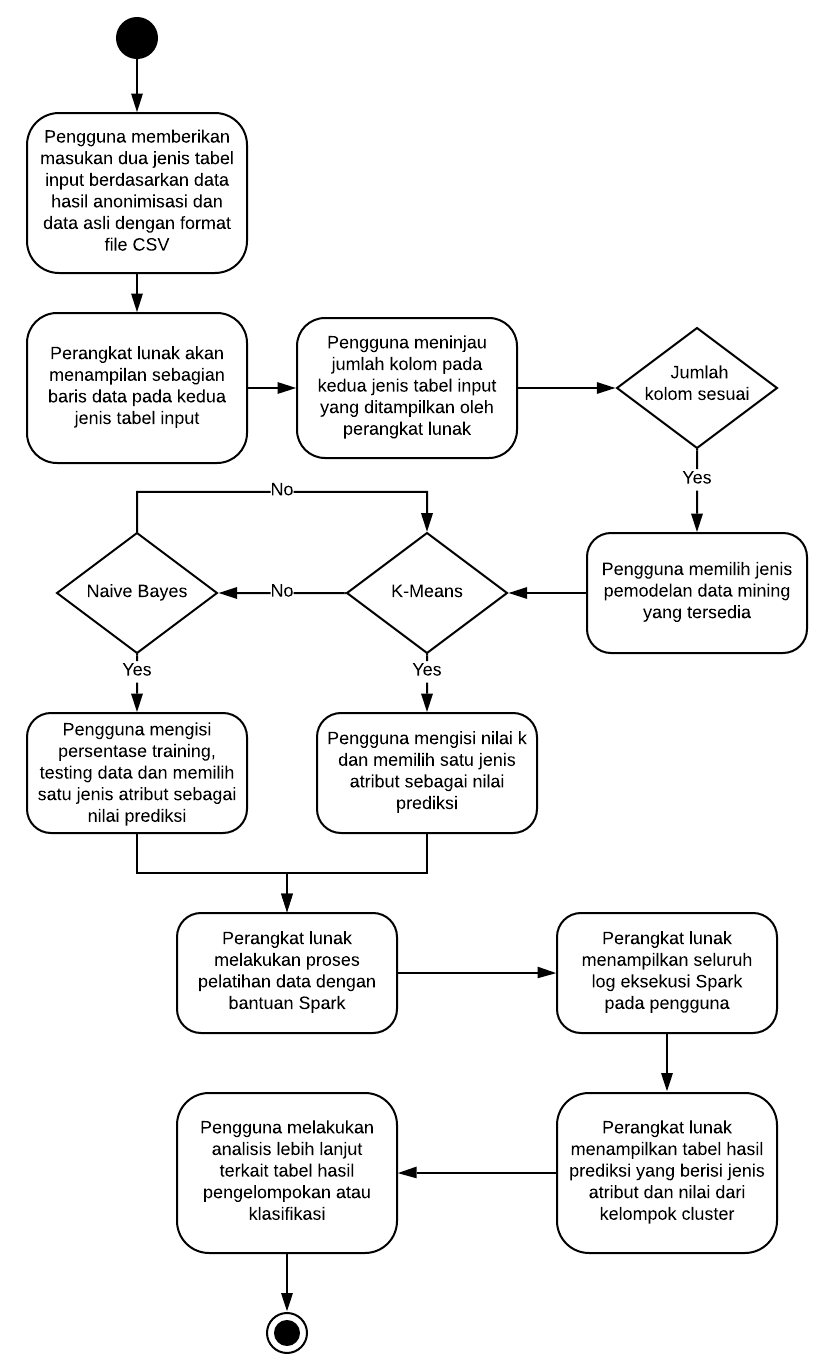
\includegraphics[scale=0.8]{pl_analisis}
	\caption{Diagram Aktifitas Analisis Data}
	\label{fig:pl_analisis}
\end{figure}
		
		
		
\end{enumerate}

\section{Pencapaian Rencana Kerja}
Langkah-langkah kerja yang berhasil diselesaikan dalam Skripsi 1 ini adalah sebagai berikut:
\begin{enumerate}
\item Mempelajari teknik-teknik dasar {\it data mining}.
\item Mempelajari algoritma {\it Greedy K-member clustering}.
\item Mempelajari konsep Hadoop, Spark, dan Spark MLlib. 
\item Melakukan instalasi dan konfigurasi Spark pada {\it cluster} Hadoop.
\item Mempelajari bahasa pemrograman Scala pada {\it framework} Spark.
\item Melakukan studi dan eksplorasi teknik-teknik dasar {\it data mining} pada Spark MLlib.
\item Mencari dan mengumpulkan data studi kasus.
\item Menulis dokumen skripsi.
\end{enumerate}



\section{Kendala yang Dihadapi}
%TULISKAN BAGIAN INI JIKA DOKUMEN ANDA TIPE A ATAU C
Kendala - kendala yang dihadapi selama mengerjakan skripsi :
\begin{itemize}
	\item Spark tidak dapat menangani data input XML.
	\item Skripsi ditempuh bersamaan dengan matakuliah lain.
	\item Pandemi COVID-19 di Indonesia mengganggu fokus pengerjaan skripsi.
\end{itemize}

\vspace{1cm}
\centering Bandung, \tanggal\\
\vspace{2cm} \nama \\ 
\vspace{1cm}

Menyetujui, \\
\ifdefstring{\jumpemb}{2}{
\vspace{1.5cm}
\begin{centering} Menyetujui,\\ \end{centering} \vspace{0.75cm}
\begin{minipage}[b]{0.45\linewidth}
% \centering Bandung, \makebox[0.5cm]{\hrulefill}/\makebox[0.5cm]{\hrulefill}/2013 \\
\vspace{2cm} Nama: \pembA \\ Pembimbing Utama
\end{minipage} \hspace{0.5cm}
\begin{minipage}[b]{0.45\linewidth}
% \centering Bandung, \makebox[0.5cm]{\hrulefill}/\makebox[0.5cm]{\hrulefill}/2013\\
\vspace{2cm} Nama: \pembB \\ Pembimbing Pendamping
\end{minipage}
\vspace{0.5cm}
}{
% \centering Bandung, \makebox[0.5cm]{\hrulefill}/\makebox[0.5cm]{\hrulefill}/2013\\
\vspace{2cm} Nama: \pembA \\ Pembimbing Tunggal
}
\end{document}

